\chapter{Nuclear Models and Nuclear Processes}
\label{chapter-nuclear-physics}

Atomic nuclei are complex systems which would be very hard, if not impossible, to describe in terms of their individual components.\footnote{As K. Krane points out in his book ``Introductory nuclear physics'', it would take about \(50!\approx10^{64}\) ``instructions'' to describe a nucleus with \(A=50\), much more than needed to describe how to build an exact replica of a French colonial house.} One therefore needs to describe a nucleus in terms of a few collective \emph{static} properties, such as its radius and binding energy, and of a few \emph{dynamic} properties which describe its decays. The challenge is to find models of what happens inside the nucleus which are accurate at reproducing experimental observations.

\section{Towards a model of the nucleus}
The development of nuclear models became necessary after the various observations of the emission of radiation, with kinetic energies of the order of a few \si{MeV} (about $10^6$ times greater than the typical chemical reactions scales) and different electric charges. 
The results of Rutherford-like experiments support the hypothesis that all positive charges within an atom are concentrated inside the nucleus. The nucleus itself is composed by protons and neutrons, collectively called as \emph{nucleons}, particles that are held together by a new force, the \emph{strong force}.
As shown in Fig.~\ref{fig:RutherfordScatteringBreakdown}, the striking aspect of the results of the measurements of Rutherford scattering at various energies is that, within a large energy range, there is no deviation from the cross section one would expect if all positive charges were concentrated in a single point. This means that whatever the force that binds the nucleus together, if the $\alpha$ particles have sufficiently low energy that they are deviated by the electromagnetic force, then the strong interaction must be short-ranged. 
As the kinetic energy of the $\alpha$ particles is increased above a certain threshold (in the figure, when \(T\approx\SI{30}{MeV}\)) there is a clear break in the cross section, which deviates from the Coulomb result and starts falling sharply.

%{\bf \color{red} To be completed}


\subsection{Nuclei dimensions}
In the Rutherford experiment the dimension of the nucleus cannot be resolved. It can be estimated using $\alpha$ radiation, which has a typical energy of $T_\alpha \sim \SI{5}{MeV}$, and therefore particle momenta $p_\alpha \sim \sqrt{2m_\alpha T_\alpha} \sim 200$MeV (as $\alpha$ particles are not relativistic at 5 MeV).

Assuming that the $\alpha$ particle is confined within the nucleus before being emitted, its momentum can be very roughly approximated as being of at least the same order of the uncertainty with which it is measured, $p_\alpha = \Delta p$. The indetermination principle\footnote{In natural units and neglecting the factor \(1/2\) - we are interested in orders of magnitude here...} states that $\Delta x \Delta p \sim 1$, therefore $\Delta x \sim \frac{1}{\Delta p}$, which means $\Delta x \approx \SI{1}{fm}$. We have already seen that at low momentum the nuclear cross-sections can be well approximated by collisions between rigid spheres. The approximation of spherical symmetry is a good approximation. Quantum mechanics tells us we cannot really expect the nucleus to sharply ``end'' after some distance, so there is no unique definition of the nuclear radius. Several methods to evaluate it have been developed, for example:
\begin{itemize}
    \item measurement of the scattering with electrons, where the distribution of the cross-section as a function of the momentum transferred to the nucleus can be extended\footnote{One can see the spatial distribution of charges inside the nucleus as the Fourier transform of the momentum distribution.} to the spatial distribution of the charges inside the nucleus;
    \item measurement of the emission spectrum of \(X\) rays by the atomic electrons, where the internal orbitals are influenced by the finite dimensions of the nucleus.
\end{itemize}
The subtle difference between the many experimental techniques arises from the fact that each of them may be sensitive to the distribution of either the \emph{nuclear charge} or  the \emph{nuclear matter}, depending on whether probe particles interact with the nucleus through the electromagnetic or  the strong interaction.

However, all these methods yield results of the same order, and in particular show that the  volume of a nucleus is proportional to its mass number \(A\). If we approximate the nucleus as a sphere of radius \(R\), we'll therefore have
\begin{equation*}
    \frac{4}{3}\pi R^3\propto A,
\end{equation*}
and therefore
\begin{equation*}
    R = R_0 A^{\frac{1}{3}},\,\,\,\,\,\,\mbox{with } R_0 \sim 1.2 \mbox{fm}.
\end{equation*}

One needs of course to keep in mind this is an approximation -- as in the case of atoms, one should not think of the nucleus as a sphere (or other distribution) with an abrupt boundary. In the end, both the Coulomb and strong potentials extend to infinity...

\subsection{Binding energy and nuclear mass}
If nuclei exist, they must live in a favourable energetic condition, which allows them to exist as \emph{bound states}. Any reasonable nuclear model should be able to quantitatively explain the existence of given nuclei and their stability.

The \emph{binding energy} of a nucleus is defined as the difference of the masses of its \(A\) constituents,
\begin{equation*}
    M_\text{nucleus}c^2 = \sum_{h=1}^{A}m_hc^2 - E_L,
\end{equation*}
where $E_L$ is the binding energy and the index \(h\) runs over all nucleons. \(E_L\) can therefore be obtained experimentally by measuring masses, for example using mass spectrometry.

For the simplest nucleus, deuterium $_{\tiny{1}}^{\tiny{2}}\mbox{H}$, we have
\begin{equation*}
    E_L^{_{\tiny{1}}^{\tiny{2}}\mbox{H}} = m_p + m_n - M(_{\tiny{1}}^{\tiny{2}}\mbox{H}) = 2.225\,\mbox{MeV}.
\end{equation*}
For an $\alpha$ particle ($_{\tiny{2}}^{\tiny{4}}\mbox{He}$) we have
\begin{equation*}
    E_L^{_{\tiny{2}}^{\tiny{4}}\mbox{He}} = 2m_p + 2m_n - M(_{\tiny{2}}^{\tiny{4}}\mbox{He}) = 28.3\,\mbox{MeV}.
\end{equation*}
It is observed that for low \(A\), the binding energy per nucleon increases with \(A\). For nuclei with $A > 12$ (i.e. elements after carbon in the periodic table) the binding energy is in good approximation proportional to the number of the constituent nucleons,
\begin{equation*}
    \frac{E_L}{A} \sim \mbox{const} \sim \SI{8}{MeV} /\text{nucleon}.
\end{equation*}

The mass of a nucleus is always lower than the mass of its constituents, and the energy difference is the binding energy: one writes
\begin{equation*}
    M(A,Z) < Zm_p + (A-Z)m_n.
\end{equation*}
This fact guarantees the \emph{stability} of the nucleus. The average binding energy per nucleon is shown in Figure \ref{nuclear-physics-fig:1} as a function of the number of nucleons in the nucleus.
\begin{figure}[h]
    \centering
    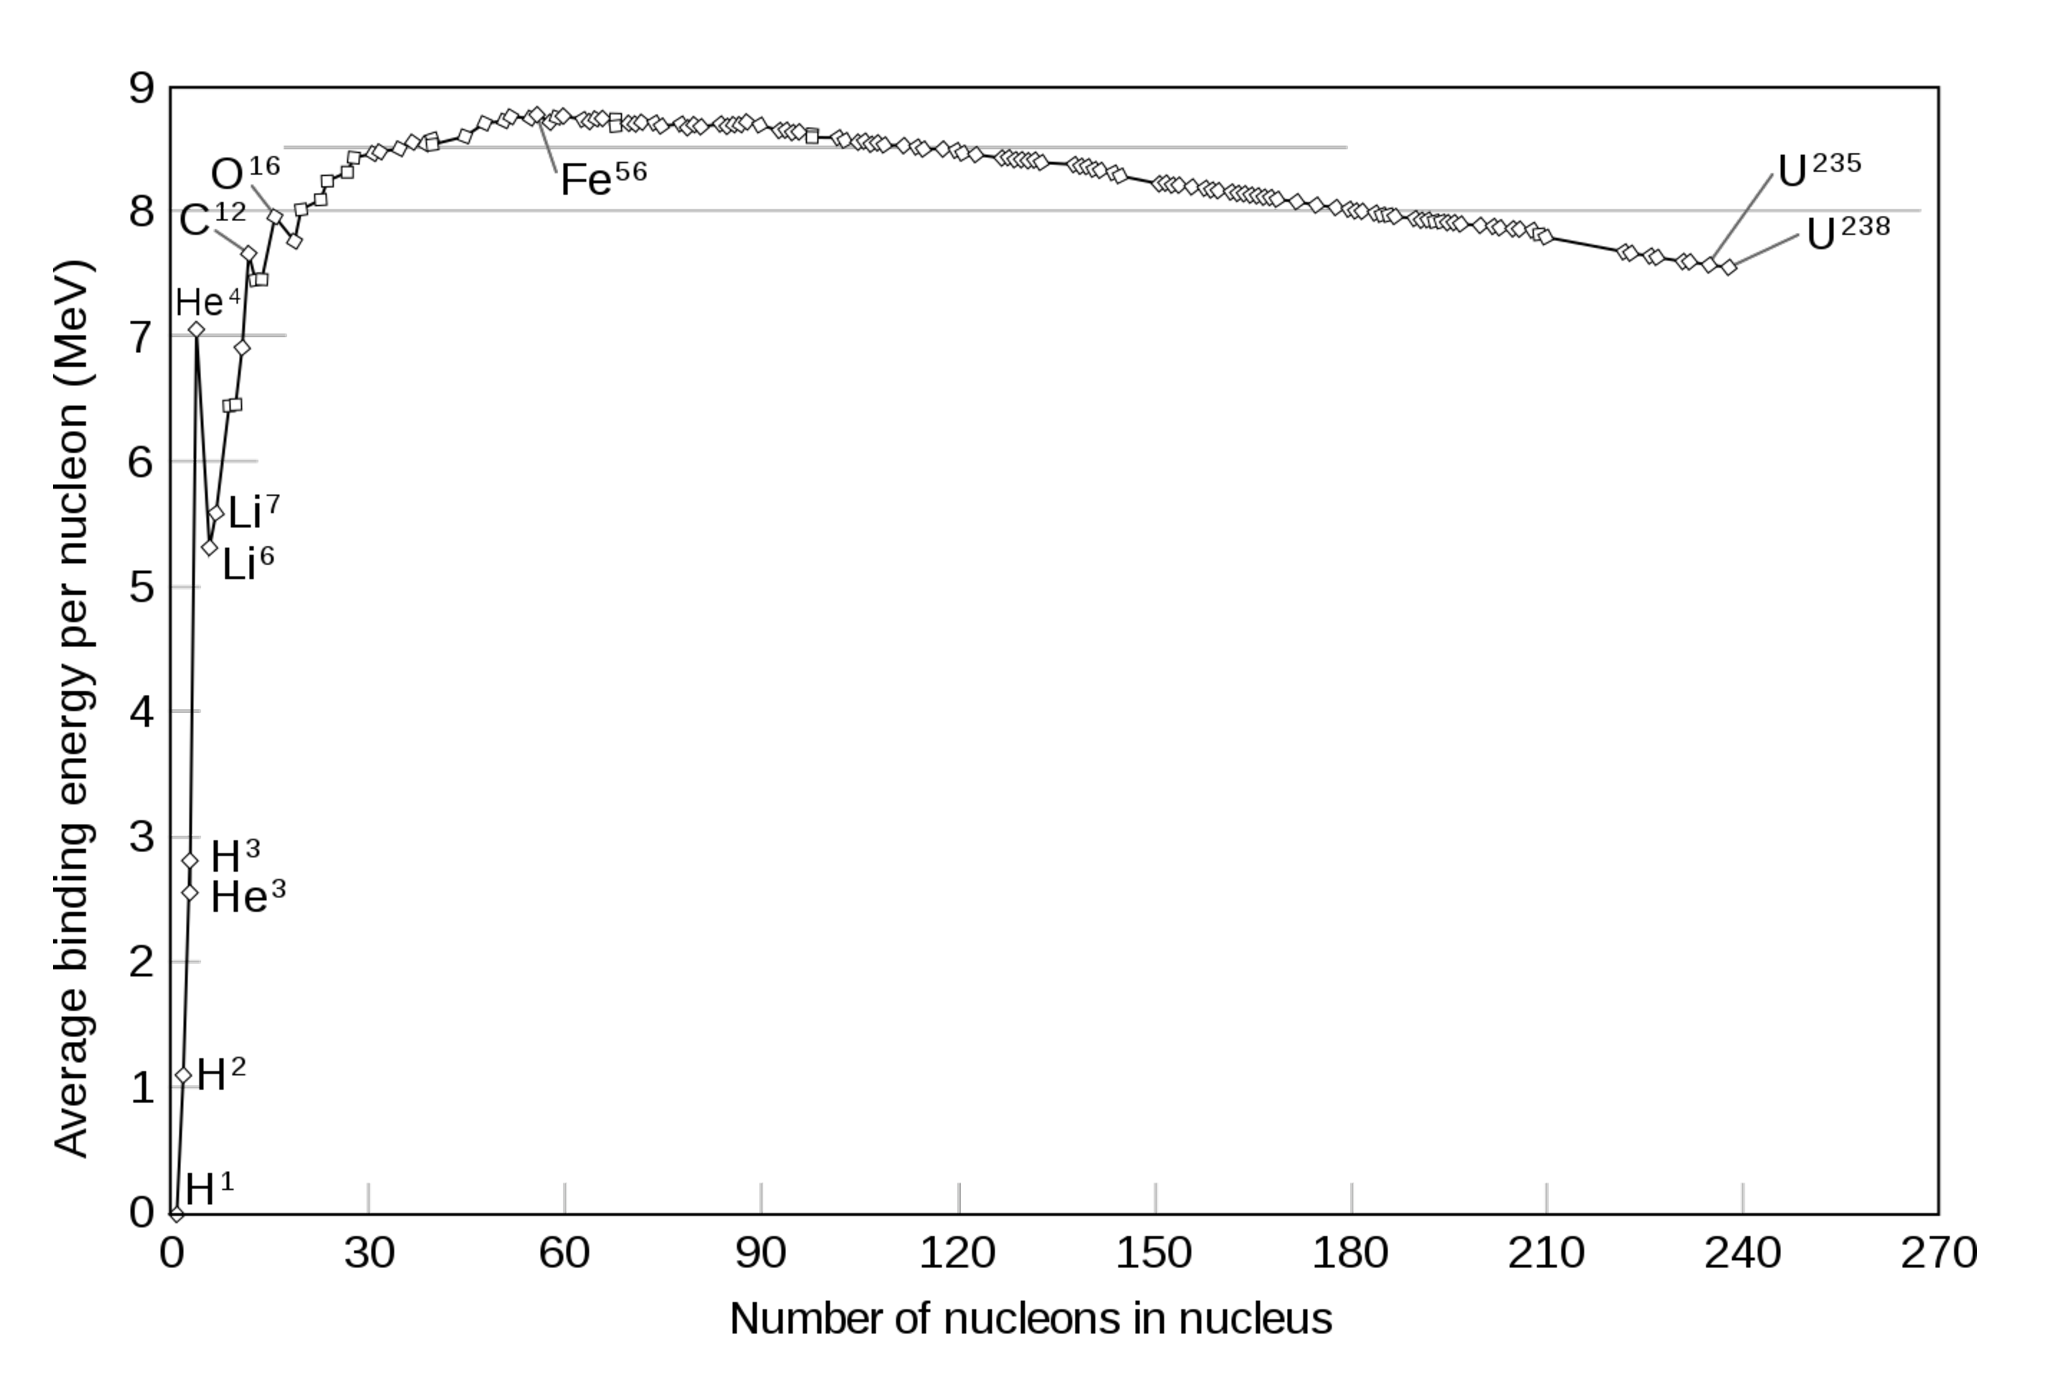
\includegraphics[scale=0.25]{Figures/nuclear-physics-fig1}
    \caption{Binding energy per nucleon as a function of the number of nucleons in the nucleus.}
    \label{nuclear-physics-fig:1}
\end{figure}

Different species of nuclei are called \emph{nuclides}, a term which identifies a configuration with a given number of protons \(Z\) and of neutrons \(A-Z\)). Nuclides which share the same atomic number \(Z\) but have different \(A\) are called \emph{isotopes} (e.g. \(_6^{12}C\), which makes \(98.9\%\) of carbon on the Earth, vs \(_6^{13}C\), with \(1.1\%\) abundance), while nuclides with the same \(A\) but different \(Z\) are called \emph{isobars} (e.g. \(_{18}^{40}Ar\) and \(_{19}^{40}K\)).
Nuclides with the same \(A-Z\) are instead called \emph{isotones}.

\subsection{Atomic masses}
The atomic mass\footnote{Usually denoted in nuclear physics textbooks with a lower-case \(m\)} instead includes the mass of the electrons and their binding energy:
\begin{equation*}
    m(\mbox{A,Z}) = M(\mbox{A,Z}) + \mbox{Z}m_e - \mbox{B}_e(\mbox{Z})/c^2,
\end{equation*}
and is expressed in atomic mass units, or unified mass units, (\si{u}), where \(\SI{1}{u}\) is defined\footnote{To be precise, as ``\(1/12\) of the mass of a free \(^{\tiny{12}}C\) atom, at rest and in its ground state'' (Bureau International des Poids et Mesures).} as \(1/12\) of the mass of a $^{\tiny{12}}C$ atom,
\begin{equation*}
    \SI{1}{u} = \SI{931.49}{MeV/c^2} =\SI{1.6605e-27}{kg}.
\end{equation*}
The Avogadro number, \(N_A = \SI{6.02e23}{mol^{-1}}\), is the number of atoms in \(12\) grams of $^{\tiny{12}}C$. 

The \emph{mass excess} is defined as the difference $m(\mbox{A,Z}) - \mbox{A}\mbox{u}$.

\subsection{Nuclear interaction}
As we have seen, the strong interaction is a short-range interaction. We can therefore think of the nucleus as a system of nucleons (protons and neutrons), where:
\begin{itemize}
    \item particles interact mostly with their first neighbors;
    \item the energy of adding an additional particle does not change the energy of the system: the energy per particle is proportional to the number of particles, $E \propto A$.
\end{itemize}
For a long-range interaction, as the Coulomb interaction, each particle would interact with all the other particles (as shown in Figure \ref{nuclear-physics-fig:2}), and therefore the energy of a particle is $E_{n+1} \propto E_{n}$, therefore the total energy will be proportional to \(A(A-1)\).
\begin{figure}
    \centering
    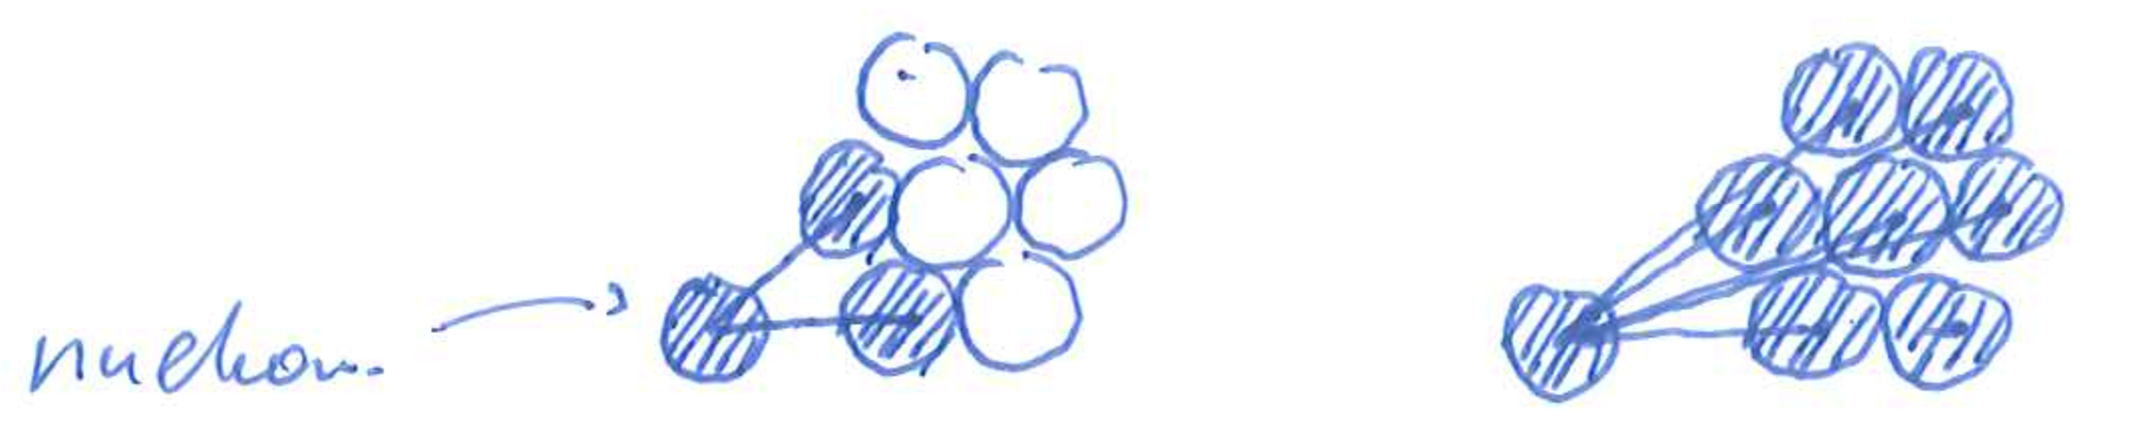
\includegraphics[scale=0.25]{Figures/nuclear-physics-fig2}
    \caption{Short-range interaction (left) versus long-range interaction (right)}
    \label{nuclear-physics-fig:2}
\end{figure}

A few experimental facts constrain our search for a quantitative description of nuclear interactions:
\begin{itemize}
    \item once Coulomb effects (which clearly happen only for protons) are subtracted, neutrons and protons behave similarly;
    \item stable nuclei typically have \(Z\sim A/2\) (i.e. there must be some reason why one does not observe isotopes of hydrogen with hundreds of neutrons);
    \item nucleons tend to couple together in a few stable configurations: most stable nuclides have an even number of neutrons and protons (i.e. configurations with an odd number of neutrons and an odd number of protons must be somehow disfavoured).
\end{itemize}

\section{The liquid drop model of the nucleus}
The liquid drop model has been suggested by N. Bohr in order to explain the experimental observations. It is based on two assumptions:
\begin{itemize}
    \item the nucleus is incompressible and shperical: $R \propto {A}^{1/3}$;
    \item the interaction between nucleons is short-ranged: $E_L \propto \mbox{A}$.
\end{itemize}
The model has been inspired by  liquid drops, where water molecules are held together by inter-molecular forces.

\subsection{The Bethe-Weizsaecker formula}
Across most of the range of Fig. \ref{fig:nuclear-physics3-fig1}, the binding energy is proportional to the mass number of the nucleus, $E_L(\mbox{A,Z}) \propto \mbox{A}$. If we see the nucleus as a sphere filled with nucleons, the internal nucleons have bindings in all directions. The external nucleons, which occupy a surface \(4\pi R^2\), are instead only bound towards the nucleons in the internal part of the nucleus: this results in another term
\begin{equation*}
    E_L \propto \mbox{A}^{\frac{2}{3}},
\end{equation*}
therefore we can sum up the two effects (nucleons in the bulk and nucleons at the surface) and write
\begin{equation*}
    E_L(\mbox{A,Z}) = -a_1\mbox{A} + a_2\mbox{A}^{\frac{2}{3}},
\end{equation*}
where the coefficients \(a_i\) are taken to be positive numbers, and the signs associated to each term take into account their contribution in making the nucleus more stable (negative sign) or less stable (positive sign) than an unbound state.

Protons, however, repel each other through electrostatic forces. This results in a contribution to \(E_L\) which is:\footnote{Formally, this term is the electrostatic energy of an uniformly-charged sphere.}
\begin{itemize}
    \item inversely proportional to the nucleus radius, $\propto \mbox{A}^{-\frac{1}{3}}$;
    \item proportional to the charge of the nucleus, $\propto \mbox{Z}^2$ (as the Coulomb interaction is  long-ranged).
\end{itemize}
Therefore, one could write
\begin{equation*}
    E_L(\mbox{A,Z}) = -a_1\mbox{A} + a_2\mbox{A}^{\frac{2}{3}} + a_3\frac{\mbox{Z}^2}{\mbox{A}^{1/3}},
\end{equation*}
which is the expression of the binding energy in a pure liquid-drop model.
Note that this model does not use the individual quantum properties of nucleons in any way.

To a better approximation, the binding energy expression is supplemented by two additional semi-empirical terms, which can be justified with a more complex quantum model of the nucleus and take into account:
\begin{itemize}
    \item the observed symmetry in the number of neutrons and protons ($N=A-Z\sim Z$), which (see the discussion on the shell model) is related to the quantised structure of the energy levels (and the Pauli exclusion principle), and leads to a term $\propto \frac{(\mbox{A-2Z})^2}{\mbox{A}}$;
    \item the fact that nuclides with an even \(A\) tend to be less stable if they have both \(Z\) and \(N=A-Z\) that are odd, which leads to a \emph{pairing term} \(\propto \pm a_s \mbox{A}^{-\frac{3}{4}}\), related to the magnetic interactions of nucleons, which  is \(0\) for odd \(A\), \(<0\) when \(A-Z\) and \(Z\) are even (even-even), and \(>0\) when \(A-Z\) and \(Z\) are odd (odd-odd).
\end{itemize}

All these terms gives the complete \emph{Bethe-Weizs\"acker formula} for the binding energy,
\begin{equation*}
    E_L(\mbox{A,Z}) = -a_1\mbox{A} + a_2\mbox{A}^{\frac{2}{3}} + a_3\frac{\mbox{Z}^2}{\mbox{A}^{1/3}} + a_4\frac{(\mbox{A-2Z})^2}{\mbox{A}} \pm a_5\mbox{A}^{-\frac{3}{4}}.
\end{equation*}
This formula is semi-empirical, in the sense that most terms have a justification in some model of the nucleus and nuclear interactions, and the parameters \(a_i\) are measured experimentally.
The $a_3$ coefficient can be evaluated from the potential energy contained in a uniformly-charged sphere,
\begin{equation*}
    E_p = \frac{3}{5}\frac{(\mbox{Z}e)^2}{4\pi \varepsilon_0 R},
\end{equation*}
where $R = R_0 A^{\frac{1}{3}}$, therefore
\begin{equation*}
    E_p = \frac{3}{5}\alpha \frac{\hslash c}{R_0}\frac{\mbox{Z}^2}{\mbox{A}^{\frac{1}{3}}},
\end{equation*}
where we used $\alpha = e^2 / 4\pi\varepsilon_0\hslash c$.
Therefore,
\begin{equation*}
    a_3 \sim \frac{3}{5}\alpha\frac{\hslash c}{R_0} \sim 0.7\,\mbox{MeV}.
\end{equation*}
The other coefficients are greater: they are found to be
\begin{itemize}
    \item $a_1 \sim 16\,\mbox{MeV}$,
    \item $a_2 \sim 18\,\mbox{MeV}$,
    \item $a_3 \sim 0.7\,\mbox{MeV}$,
    \item $a_4 \sim 24\,\mbox{MeV}$,
    \item $a_5 \sim 34\,\mbox{MeV}$.
\end{itemize}

The minimum of the binding energy (i.e. the most favoured configuration in terms of atomic and mass numbers) is obtained for
\begin{equation*}
    \frac{\partial E_L (\mbox{A,Z})}{\partial \mbox{Z}} = 2a_3\frac{\mbox{Z}}{\mbox{A}^{\frac{1}{3}}} - 4a_4\frac{\mbox{A-2Z}}{\mbox{A}} = 0,
\end{equation*}
which defines the relation
\begin{equation*}
    \mbox{Z} = \frac{2a_4\mbox{A}}{a_3A^\frac{2}{3}+4a_4}.
\end{equation*}
This relation defines the \emph{valley of stability}, which shows two regimes:
\begin{itemize}
    \item for small \(A\) (since $a_3$ is small) it can be approximated as $\mbox{Z} \sim \frac{\mbox{A}}{2}$;
    \item for high \(A\) it can be approximated as $\mbox{Z} \sim \frac{2a_4}{a_3}\mbox{A}^{\frac{1}{3}}$.
\end{itemize}
Both approximations are in good agreement with observation for light and heavy stable nuclei.

\begin{figure}
    \centering
    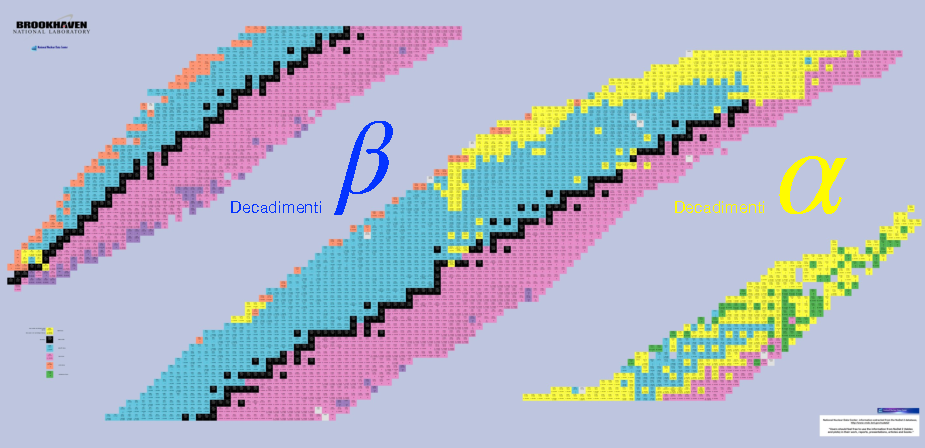
\includegraphics[scale=0.70]{Figures/nuclear-physics-fig3}
    \caption{Valley of stability. Source https://www.nndc.bnl.gov/nudat2/.}
    \label{nuclear-physics-fig:3}
\end{figure}

If we evaluate the binding energy $E_L$ for isobars (i.e. for a given value of \(A\)), we find a parabola for nuclei with odd \(A\), and two parabolas for nuclei with even \(A\). In the first case, there is only one stable isobar for a fixed (odd) \(A\), which can be reached through \(\beta^+\) or \(\beta^-\) decays. In the second case, instead, there are many stable isobars for a fixed (even) \(A\).

From the Bethe-Weizs\"acker formula, one can also see\footnote{One should express the mass of a nuclide in terms of \(Z,A\) and of the binding energy, and then require that the Q-value of each decay is positive.} that for \(A\) higher than about \(150\) nuclei are predicted to be stable against the emission of \(\alpha\) particles, while for \(A\) higher than about \(90\) nuclei can decay by fission into two lighter nuclei (\emph{fragments}) of approximately the same mass number.

\section{Fermi gas model}
The Fermi gas model is a first attempt at including quantum effects in a nuclear model. It assumes that protons and neutrons confined in a potential well with spherical symmetry in the nucleus region, with radius $R = R_0 A^{1/3}$.
\begin{figure}[h]
    \centering
    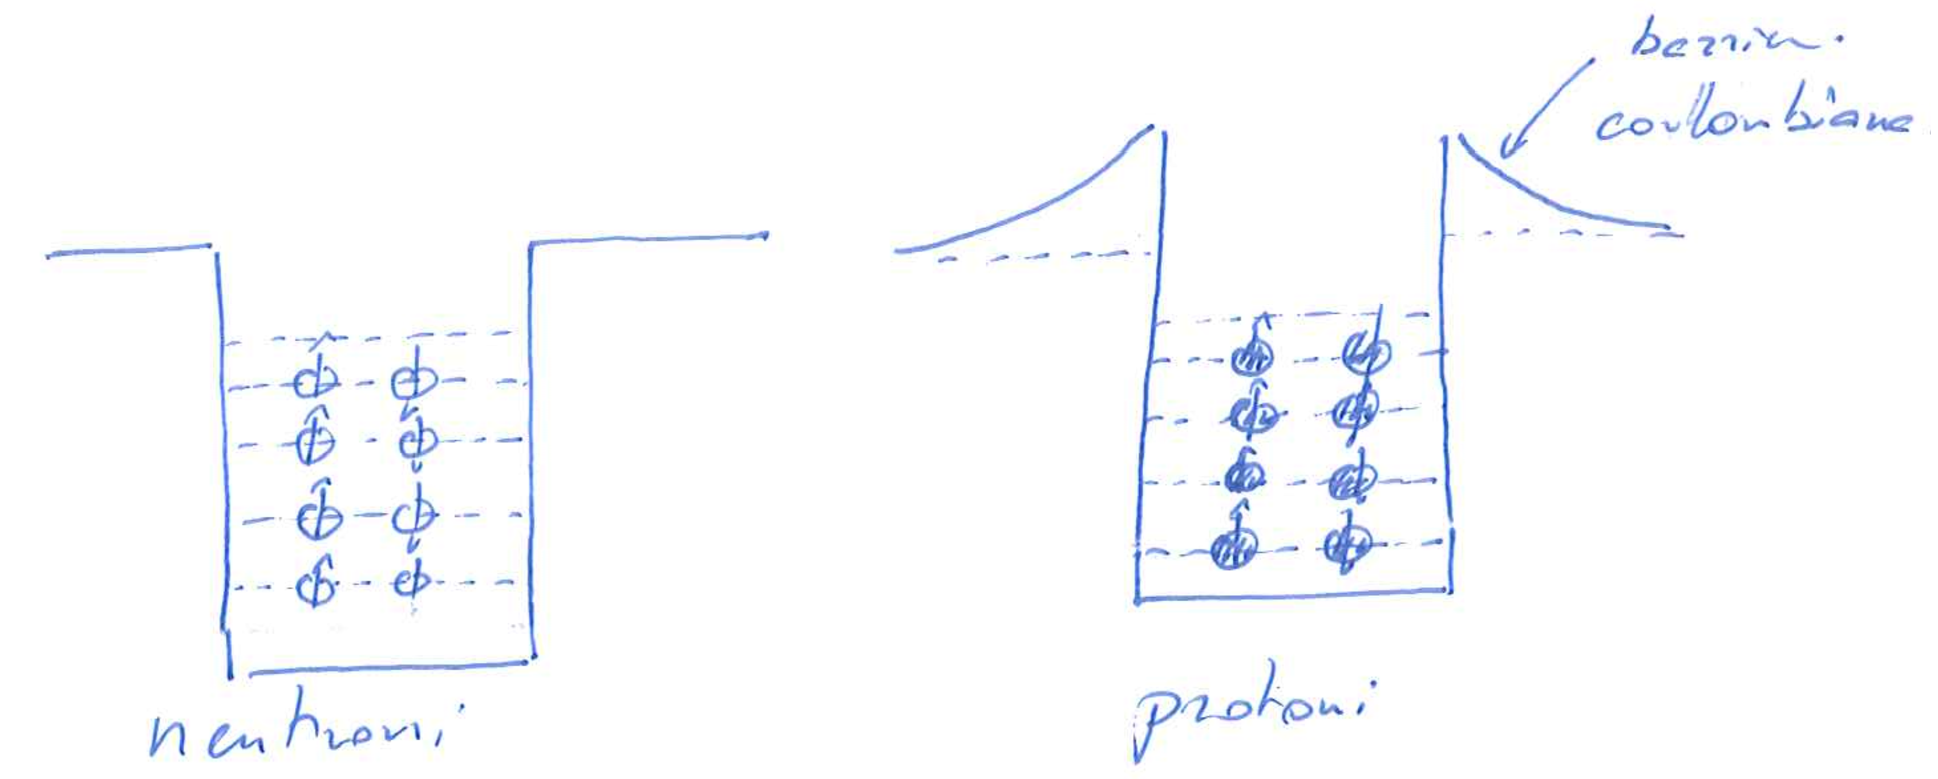
\includegraphics[scale=0.35]{Figures/nuclear-physics-fig9}
    \caption{Fermi gas model representation of nucleons within a potential well.}
    \label{nuclear-physics-fig:9}
\end{figure}

If we ignore spin, the number of states neutrons (or protons) can occupy can be calculated starting from the phase space element
\begin{equation*}
    dn = \frac{4\pi p^2dpV}{(2\pi\hslash)^3},
\end{equation*}
which must be integrated over the particle momentum, which will have a maximum value $p_F$ (\emph{Fermi momentum}), i.e. the maximum momentum of the fundamental state. In formulas, we have
\begin{equation*}
    n = \int_0^{p_F} \frac{4\pi p^2 dp V}{(2\pi\hslash)^3} = \frac{Vp_F^3}{6\pi^2\hslash^3}.
\end{equation*}
But neutrons and protons have spin \(1/2\), so we must take into account the fact that there are two possible particle states for each energy state, separated for neutrons and protons. For neutrons, we have a number of states
\begin{equation*}
    \mbox{N} = \mbox{A} - \mbox{Z} = 2n = \frac{Vp_F^3}{3\pi^2\hslash^3},
\end{equation*}
and for protons
\begin{equation*}
    \mbox{Z} = \frac{Vp_F^3}{3\pi^2\hslash ^3}.
\end{equation*}

If we approximate the nucleus as a sphere as discussed before, 
\begin{equation*}
    V = \frac{4}{3}\pi R^3 = \frac{4}{3}\pi R^3_0 \mbox{A}
\end{equation*}
in the approximation $\mbox{Z} \sim N \sim \frac{\mbox{A}}{2}$ we obtain
\begin{equation*}
    \frac{\mbox{A}}{2} = \frac{4}{3}\frac{\pi R^3_0}{3\pi^2\hslash^3}\mbox{A}p_F^3,
\end{equation*}
which leads to
\begin{equation*}
    p_F = \frac{\hslash}{R_0}\left(\frac{9\pi}{8}\right)^{\frac{1}{3}}\sim \SI{250}{MeV/c},
\end{equation*}
and the \emph{Fermi energy} will be\footnote{Again, at these momenta the non-relativistic approximation is accurate.}
\begin{equation*}
    E_{F} = \frac{p_F^2}{2m_N} \sim \SI{33}{MeV},
\end{equation*}
which represents the energy of the highest-energy occupied nucleon state. The sum of the Fermi energy and of the binding energy of the nucleus (which, as we have seen, is approximately \SI{8}{MeV} per nucleon for sufficiently heavy nuclides) will give the depth of the potential well of the Fermi gas model.

\begin{figure}[h]
    \centering
    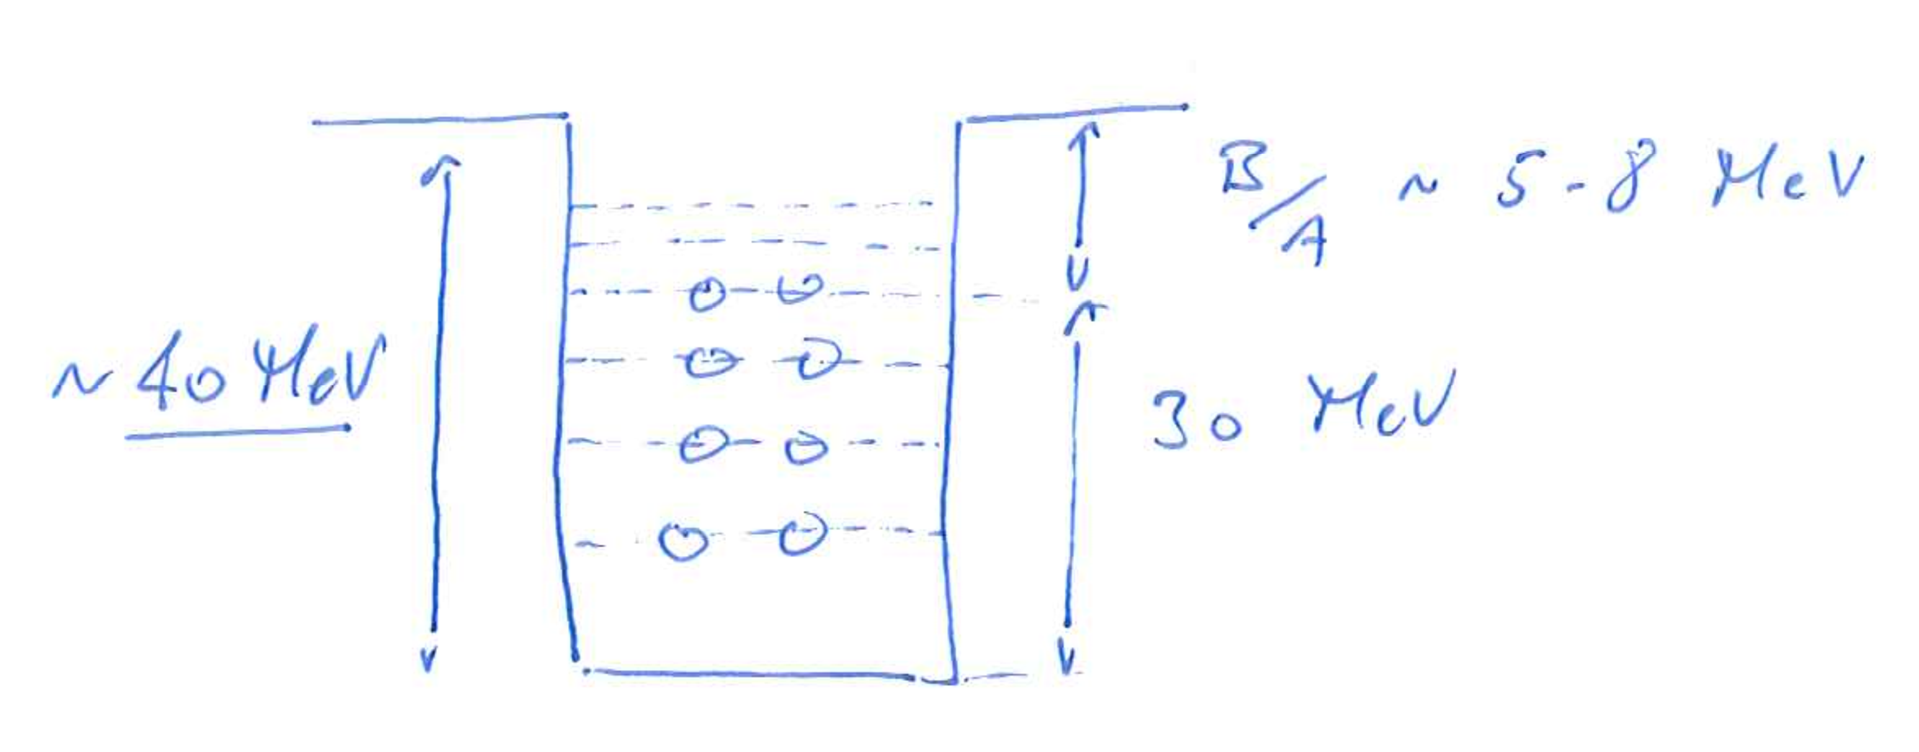
\includegraphics[scale=0.3]{Figures/nuclear-physics-fig10}
    \caption{Pothole.}
    \label{nuclear-physics-fig:10}
\end{figure}

\section{Shell model and Magic Numbers}
The atomic model of Bohr-Sommerfeld, based on a Coulombian potential with spherical symmetry (with a well defined centre: the nucleus) is based on the laws of quantisation of the angular momentum and on the Pauli exclusion principle. It is able to reproduce the phenomenology of the atoms.
The atomic energy levels are identified by the quantum numbers
\begin{equation*}
    |n, l, m\rangle
\end{equation*}
where \(n = 1, 2, 3, \dots, l = 0, \dots, n-1\) and \(m = -l, \dots, l\). The number of electrons per level is given by
\begin{equation*}
    \mbox{Z}_n = \sum_{l = 0}^{n-1} 2(2l+1) = 2n^2.
\end{equation*}
The elements with complete levels, \(Z = 2, 10, 18, 36, \dots\), are the noble elements (helium, neon, argon, etc), and have a total angular momentum \(J = 0\) and a high binding energy.

Can we proceed in an analogous way in the case of nuclei? A similarity is suggested from the experimental evidence that there are particular nuclide configurations which are stable. These are obtained for the \textit{magic numbers} of number of neutrons (\(N = A - Z\)) equal to \(2, 8, 20, 28, 50, 82, 126\). These nuclei have particularly large binding energy, and a satisfactory model of the nucleus should be able to reproduce this experimental fact. It would be actually tempting to explain the sharp discontinuity in the binding energy (or, equivalently, in the relative abundance of nuclides) in correspondence of the magic numbers, as the result of the filling of some nuclear shells occupied by nucleons.
\begin{figure}[h]
    \centering
    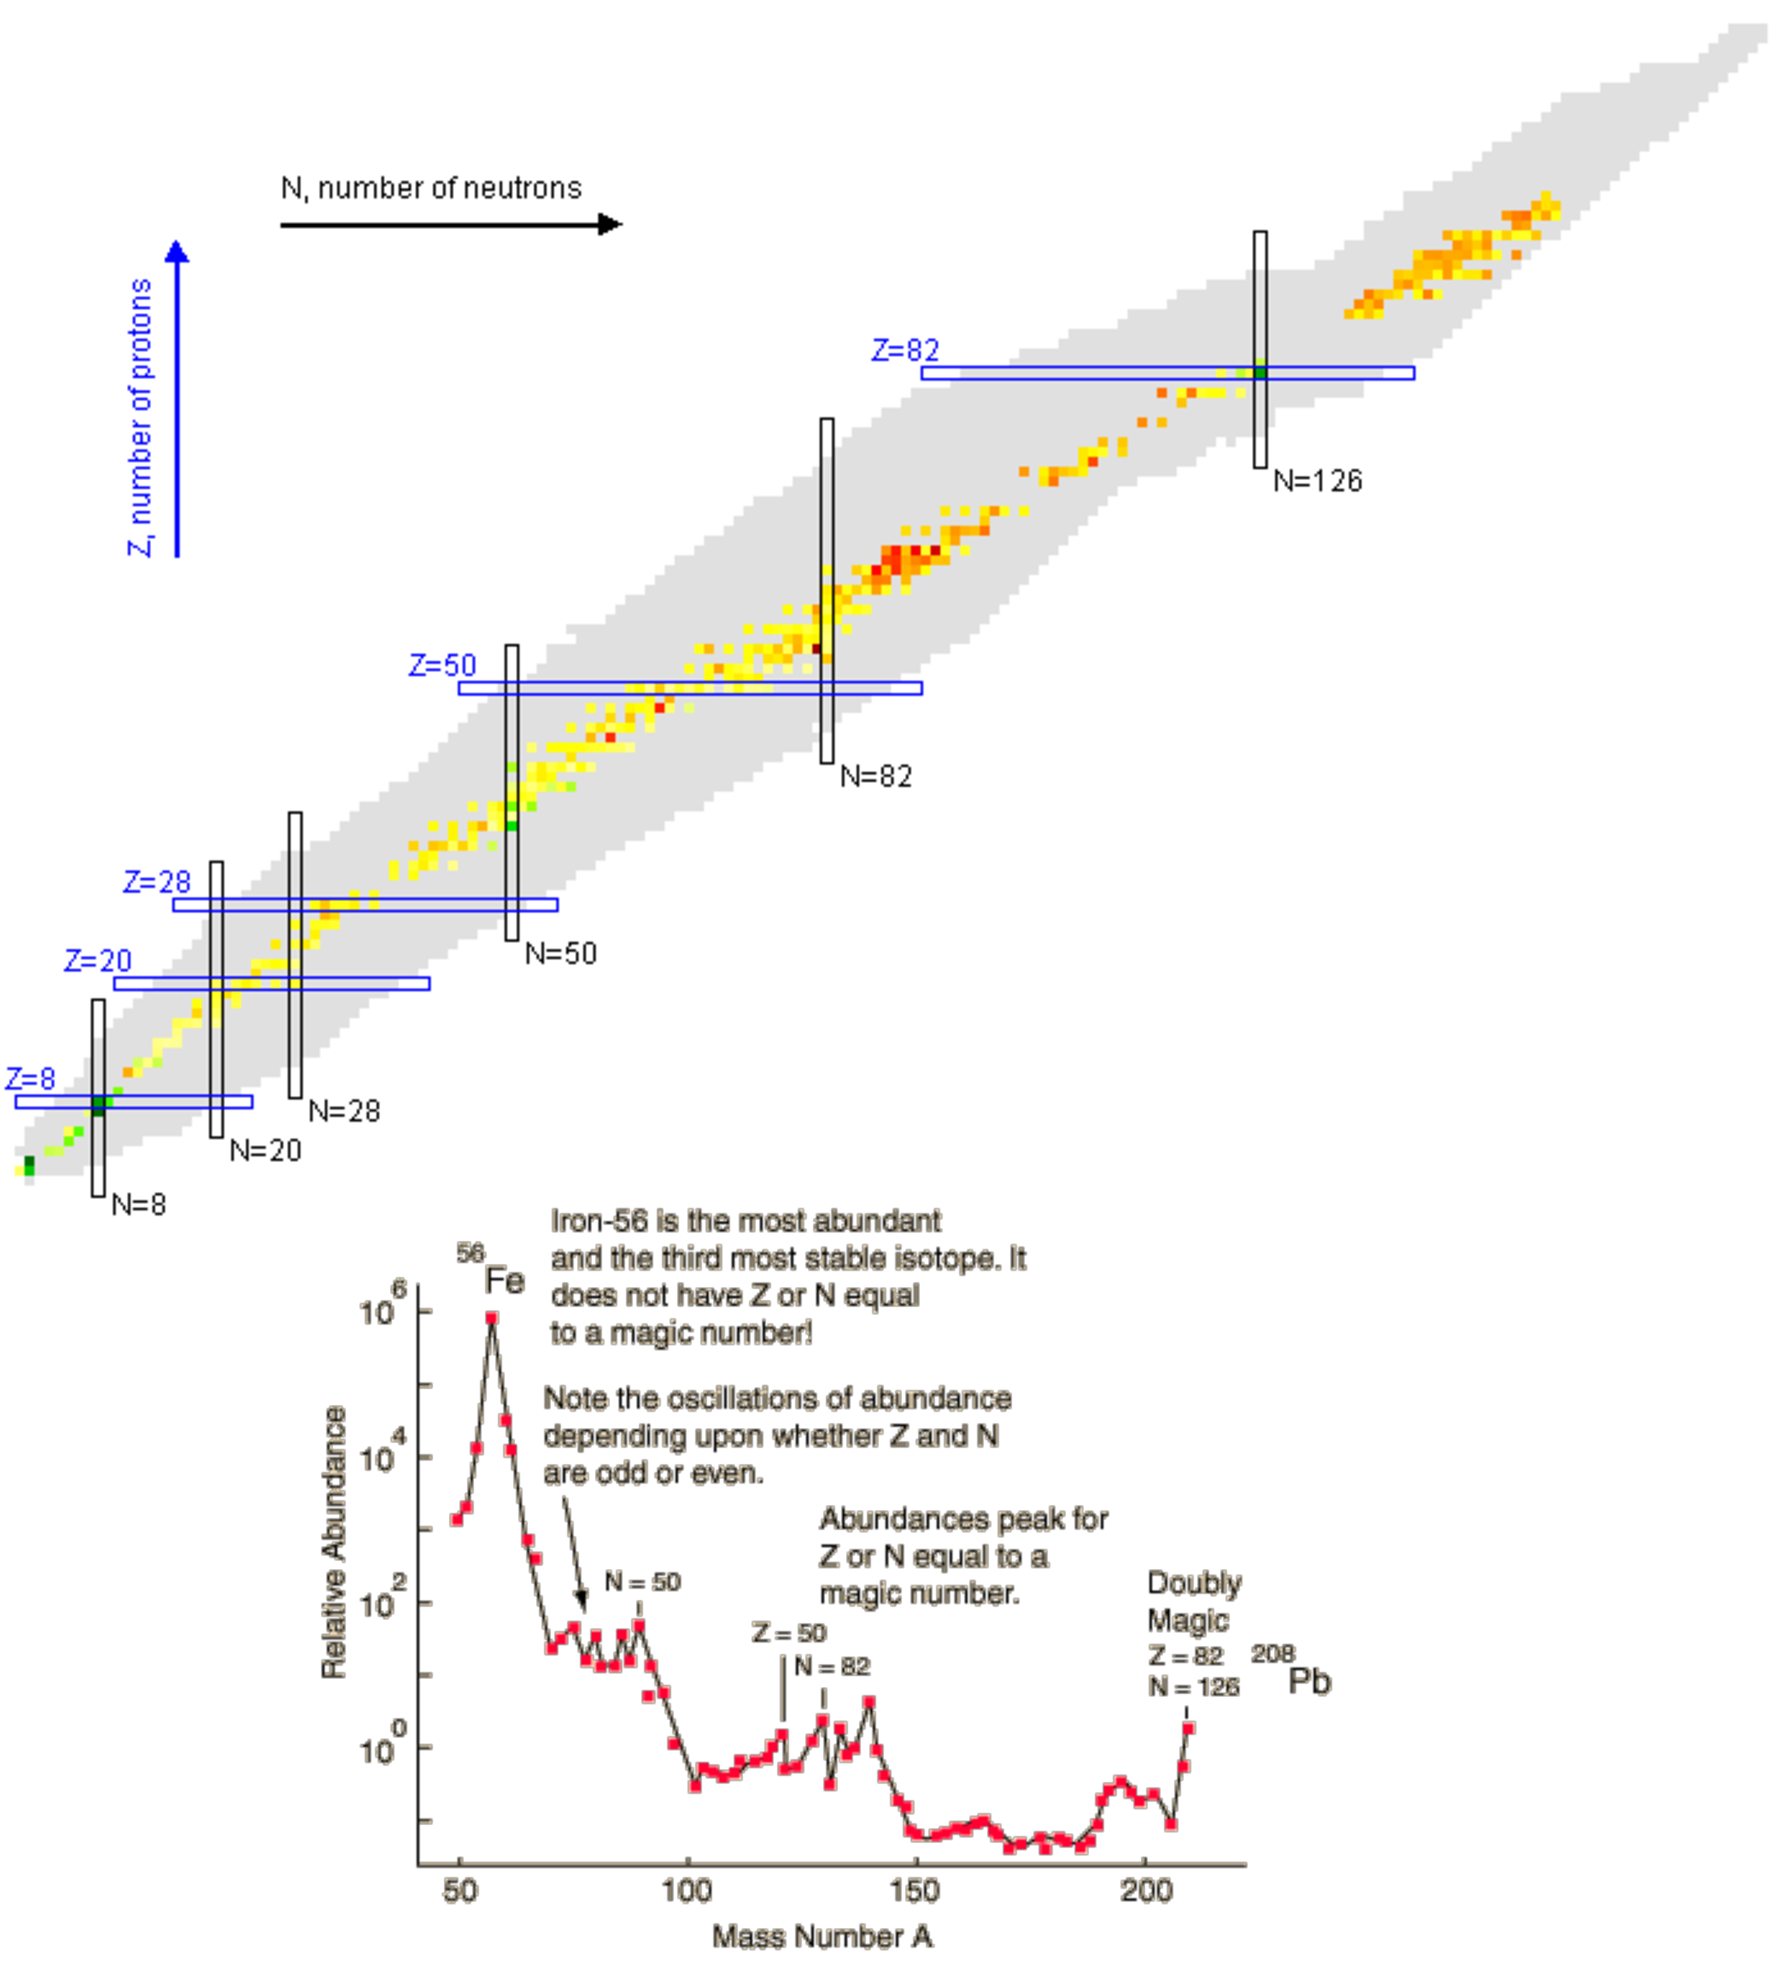
\includegraphics[scale=0.38]{Figures/nuclear-physics-fig11}
    \caption{Nuclei distribution in the \(N, Z\) plane.}
    \label{nuclear-physics-fig:11}
\end{figure}

Actually, it is not trivial to find a model which describes the nucleus: solving the Schr\"odinger equation is hard, because the nuclear potential is not known, and the symmetry centre is as easily defined as in the case of the atom. Moreover, while electrons can be regarded as relatively free from  collisions with other electrons, the nucleons occupy the nucleus in a continuous way, therefore the concept of orbital cannot be trivially ``ported'' from electrons to nucleons. Definite spatial orbits however should exist, due to the Pauli exclusion principle (nucleons are fermions).

The first (quite complex!) task is to find a model of the nuclear potential: in the shell model, one assumes that a single nucleon feels the potential due to all other nucleons. If we model this potential with an armonic potential, we get solutions which are close (parabolas) to the magic numbers. Such potential is able to reproduce only the \(N=2\), \(8\) and \(20\) nuclides, then the \(N=40\), \(70\) and \(112\) nuclides. The other magic numbers cannot be explained with an armonic potential. Similar disagreement with the observation is obtained in the case of an infinite-well potential.

The potential proposed by Woods-Saxon, 
\begin{equation*}
    V(r) = \frac{-V_0}{1+e^{(r-R)/a}},
\end{equation*}
represented in Figure \ref{nuclear-physics-fig:12}, provides a more accurate description of the nuclear interaction, but is not able to reproduce by itself the exact numbers, as it predicts \(N=2, 8, 20, 40, 58, 92\) and \(112\). The parameters \(R\) and \(a\) represent the nuclear radius and its \emph{skin thickness}, respectively; one has \(V_0\approx\SI{50}{MeV}\), \(R\approx 1.2A^{1/3}\) and \(a\approx\SI{0.5}{fm}\). The Woods-Saxon potential removes the degeneracy in the quantum number \(l\) of the major shells, but still isn't enough.
\begin{figure}[h]
    \centering
    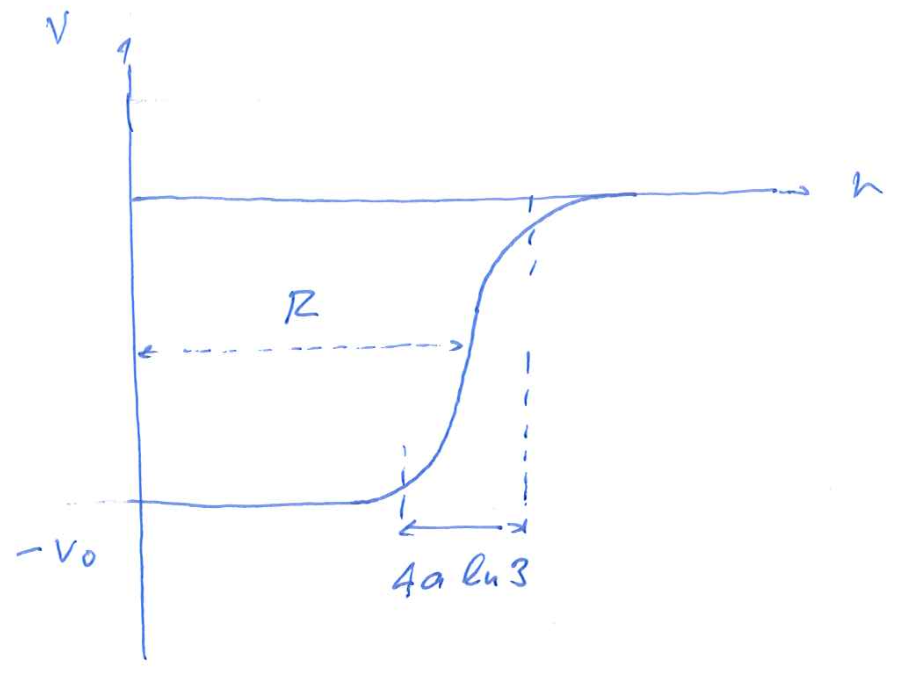
\includegraphics[scale=0.45]{Figures/nuclear-physics-fig12}
    \caption{The Woods-Saxon potential}
    \label{nuclear-physics-fig:12}
\end{figure}

Using this model, Maria Meyer and Hans Jensen (Nobel prize in 1963), with the addition of a term depending on the spin (a \emph{spin-orbit} term analogous to the one of atomic physics), managed to obtain more accurate results when compared to data. Their model uses a Woods-Saxon potential, and assumes that a nucleon-nucleon spin-orbit interaction proportional to \(\Vec{L}\cdot\Vec{S}\) exists, which is due to the nuclear interaction (not to the electromagnetic one!). The nucleons have an orbital momentum $\Vec{L}$, which can be seen from the nucleus reference frame or from the reference frame fixed with a nucleon, as shown in Figure \ref{nuclear-physics-fig:13}.
\begin{figure}[h]
    \centering
    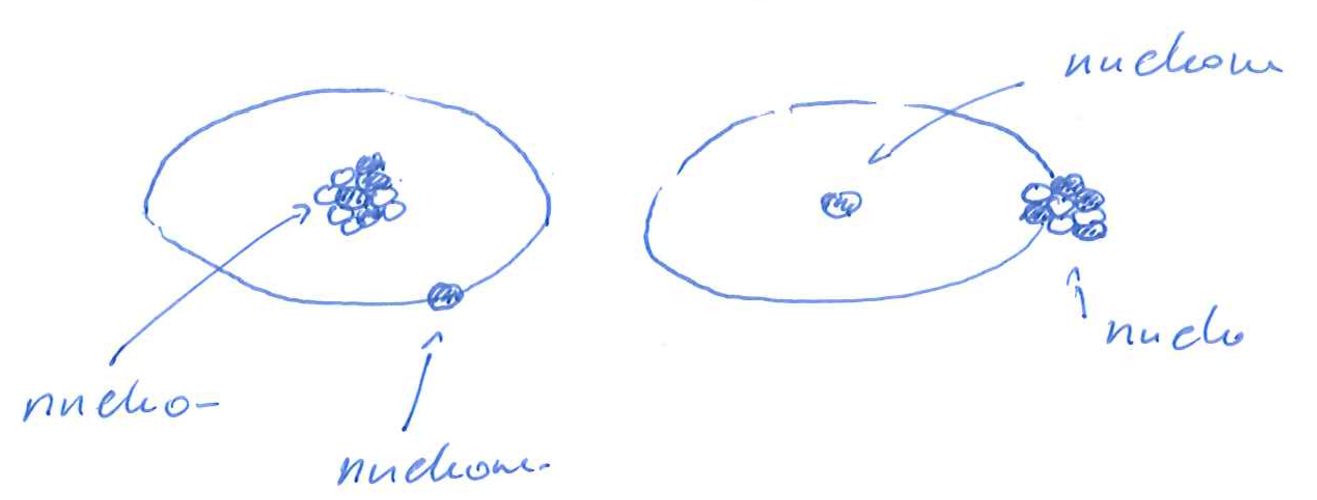
\includegraphics[scale=0.4]{Figures/nuclear-physics-fig13}
    \caption{Two ways of seeing the nucleus-nucleon system.}
    \label{nuclear-physics-fig:13}
\end{figure}
The orbital angular momentum brings a magnetic momentum, $\Vec{\mu}$, which generates a magnetic field as shown in Figure \ref{nuclear-physics-fig:14}.
\begin{figure}[h]
    \centering
    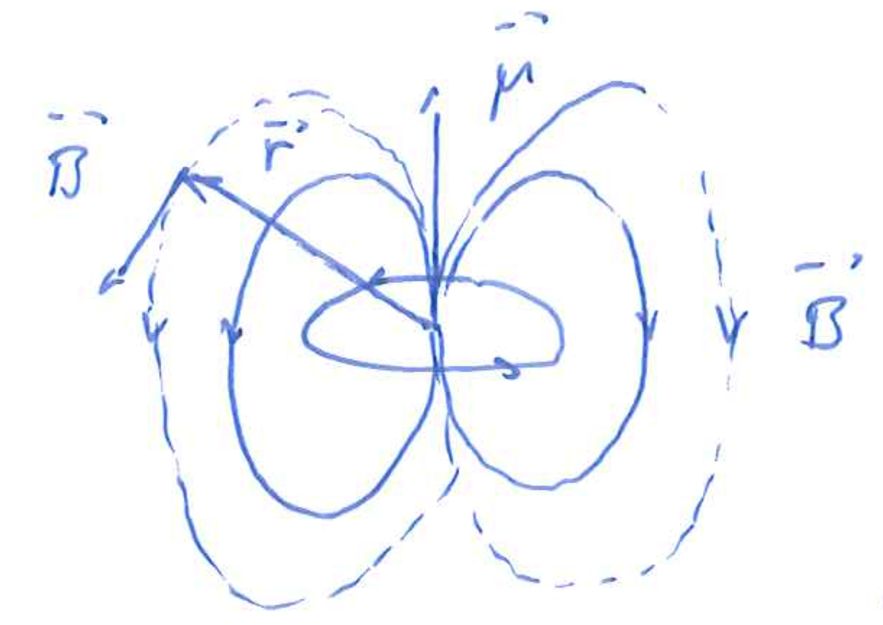
\includegraphics[scale=0.4]{Figures/nuclear-physics-fig14}
    \caption{Magnetic field generated by a magnetic momentum.}
    \label{nuclear-physics-fig:14}
\end{figure}

The magnetic field generated by a dipole in a point of space identified by the radius vector \(\Vec{r}\) is
\begin{equation*}
    \Vec{B} = \frac{\mu_0}{4\pi}\left[\frac{3\Vec{r}\cdot(\Vec{\mu}\cdot\Vec{r})}{r^5} - \frac{\Vec{\mu}}{r^3}\right],
\end{equation*}
and can alternatively be written using the unit vector $\hat{r}$ as
\begin{equation*}
    \Vec{B} = \frac{\mu_0}{4\pi}\left[\frac{3\hat{r}(\Vec{\mu}\cdot\Vec{r})-\Vec{\mu}}{r^3}\right].
\end{equation*}
The spin of the nucleon gives an additional magnetic momentum. Since the potential energy for a magnetic momentum in a field $\Vec{B}$ is 
\begin{equation*}
    U = -\Vec{\mu}\cdot\Vec{B},
\end{equation*}
the interaction between the magnetic momentum of the spin (subscript \(S\)) and the orbital magnetic momentum (subscript \(L\)) will be
\begin{equation*}
    U = -\frac{\mu_0}{4\pi}\left[\frac{3(\Vec{\mu}_L\cdot\hat{r})(\Vec{\mu}_S\cdot\hat{r}) - \mu_l\mu_S}{r^3}\right].
\end{equation*}
Given the small dimension of the nucleus (\(r\approx R\)), this term is not negligible, as $U$ is of the order of a few \si{keV} (to be compared to the case of atoms, where \(U\approx\si{meV}\).

The energy term that describes the spin-orbit interaction will be
\begin{equation*}
    U \propto \Vec{L}\cdot\Vec{S}.
\end{equation*}
With this term, the shell model is able to predict the magic numbers, i.e. the most stable configurations in terms of \(N\) and \(Z\).
In fact, similarly to the case of atomic physics, each level is split into two levels,
\begin{equation*}
    J = l + \frac{1}{2}\,\,\,\,\mbox{and}\,\,\,\,J = l - \frac{1}{2}.
\end{equation*}
 Since the total momentum operator can be written as $\hat{J} = \hat{L} + \hat{S}$, then
\begin{equation*}
    \hat{L}\cdot\hat{S} = \frac{1}{2}\left[\hat{J}^2-\hat{L}^2-\hat{S}^2\right]
\end{equation*}
therefore the separation \(\Delta\) between the levels is given by
\begin{equation*}
    \hat{L}\cdot\hat{S} = \frac{1}{2}\left[J(J+1) - l(l+1) - s(s+1)\right]
\end{equation*}
and can be expressed as
\begin{equation*}
\begin{split}
    \Delta(\hat{L}\cdot\hat{S}) & = J_{l+S}(J_{l+s}+1) - J_{l-S}(J_{l-S}+1) \\
    & = (l+\frac{1}{2})(l+\frac{3}{2}) - (l-\frac{1}{2})(l+\frac{1}{2}) = 2(l+\frac{1}{2}),
\end{split}
\end{equation*}
so the separation between the levels is increasing with \(l\), as shown in Figure \ref{nuclear-physics-fig:15}. 
\begin{figure}[h]
    \centering
    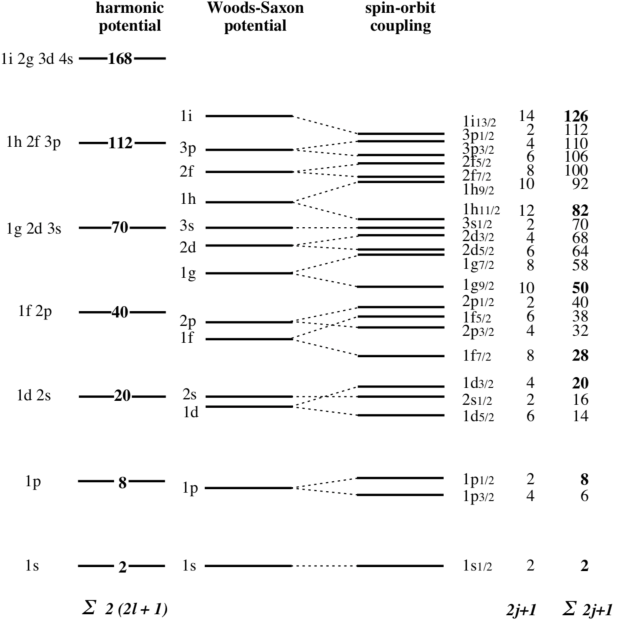
\includegraphics[scale=0.8]{Figures/nuclear-physics-fig15}
    \caption{Splitting of levels predicted by the nuclear shell model using three different potentials: the harmonic potential, the Woods-Saxon potential and the Meyer-Jensen model (which extends the latter with spin-orbit interactions).}
    \label{nuclear-physics-fig:15}
\end{figure}
This explains the magic numbers.

The nuclei in which the protons and/or neutrons cover complete states are called \emph{doubly magic}. A few of them are:
\begin{itemize}
    \item \(^{4}He\): 2 protons, 2 neutrons;
    \item \(^{16}O\): 8 protons, 8 neutrons;
    \item \(^{42}Si\): 14 protons, 28 neutrons;
    \item \(^{40}Ca\): 20 protons, 20 neutrons;
    \item \(^{48}Ca\): 20 protons, 28 neutrons;
    \item \(^{48}Ni\): 28 protons, 20 neutrons;
    \item \(^{208}Pb\): 82 protons, 126 neutrons.
\end{itemize}
They are particularly stable against decays.

\subsection{Interpreting the fourth and fifth terms of the Bethe-Weizs\"acker formula}
While the first three terms in the Bethe-Weizs\"acker formula have an empirical justification in the liquid drop model, the last two terms can be understood in terms of the shell model.

\subsubsection*{The fourth term}
We have seen as in the Bethe-Weizsaecker formula the fourth term includes the contribution of the symmetry between protons and neutrons. Keeping in mind the Pauli exclusion principle, this term can be explained by the fact that keeping the equilibrium between protons and neutrons, a favorable energy configuration can be achieved.

\subsubsection*{Spin-spin interactions and the fifth term}
In the same way of the spin-orbit interaction, there must be a spin-spin interaction term between two nearby nucleons. This term is called \textit{paring energy}, and favours the situation in which the two spins are anti-aligned, resulting in a spin-zero state.

The nuclei in which \(Z\) and \(N = A - Z\) are both even (also called even-even nuclei) have their fundamental state with $J = 0$.

From the spin-spin interactions one can deduce that the configuration on the left of Figure \ref{nuclear-physics-fig:16} is favoured, while the one on the right is disfavoured.
\begin{figure}[h]
    \centering
    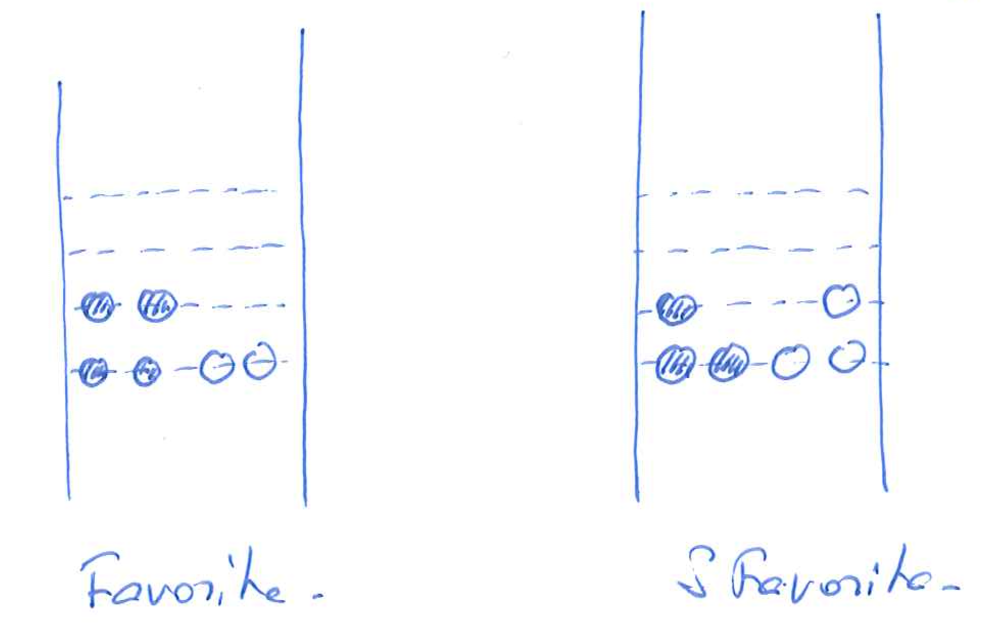
\includegraphics[scale=0.5]{Figures/nuclear-physics-fig16}
    \caption{Favoured and disfavoured conditions in a nucleus.}
    \label{nuclear-physics-fig:16}
\end{figure}
The spin-spin interaction term is
\begin{itemize}
    \item negative for even-even configurations;
    \item null for odd A;
    \item positive for odd-odd nuclei
\end{itemize}

\subsection{Isotopic spin}
We have seen that neutrons and protons have nearly the same mass, and the nuclear interactions does not distinguish between protons and neutrons.
One can therefore assume that, from the point of view of the nuclear interaction, only one kind of particle exists, the \textit{nucleon} $N$, which can be found in one of two possible states, the neutron and the proton. This implies the existence of a degree of freedom similar to spin which is identified as the \emph{isotopic spin}, or \emph{isospin}.
\begin{equation*}
    |p\rangle = \left(\begin{array}{c}
    1 \\
    0
    \end{array}\right) \,\,\,\, \text{and} \,\,\,\, |n\rangle = \left(\begin{array}{c}
    0 \\
    1
    \end{array}\right)
\end{equation*}
The eigenvalue of the squared isotopic spin operator \(\hat{I}^2\) of a nucleon $N$ is $\frac{1}{2}$, and the proton and neutron can be identified -- similarly to what is done in the case of ordinary spin -- in the basis of \(\hat{I}^2,\hat{I}_3\) as the states
\begin{equation*}
    |p\rangle = |\frac{1}{2}, +\frac{1}{2}\rangle,
\end{equation*}
\begin{equation*}
    |n\rangle = |\frac{1}{2}, -\frac{1}{2}\rangle.
\end{equation*}

Using this symmetry, we can build the shell model without differences between protons and neutrons. (In a similar way of how the Bohr-Sommerfeld model was initially not considering the spin of the electrons). The interaction that allows the interchange between protons or neutrons is the $\beta$ decay, which plays an essential role in the valley of stability.

\section{Nuclear beta decays, corroborating the nuclear models}
\label{sec:NuclearBeta}
Beta decays do not change the mass number of nuclides, but only their atomic number \(Z\), transmuting one proton in neutron (or vice-versa) via the three processes
\begin{align*}
    N(Z,A) &\to N(Z+1, A) + e^- + \bar{\nu}_e,\\
    N(Z,A) &\to N(Z-1, A) + e^+ + \nu_e,\\
    N(Z,A) + e^{-} &\to N(Z-1, A) + \nu_e, \nu_e,
\end{align*}
where the last process is called \emph{electron capture} and can happen whenever \(\beta^+\) decays are allowed.

As such, beta decays are the process via which isobars transform in each other, decaying towards more stable states with the same \(A\). For example, the processes
\begin{align*}
    _{55}^{137}Cs &\to _{56}^{137}Ba + e^- + \bar{\nu}_e,\\
    _{11}^{22}Na &\to _{10}^{22}Ne + e^+ + {\nu}_e,\\
    _{11}^{22}Na + e^-&\to _{10}^{22}Ne + {\nu}_e,
\end{align*}
correspond to different transitions in the parabola(s) of the Bethe-Weizs\"acker formula of the binding energy. If \(A\) is odd, all isobars (nuclides with the same \(A\)) lie on the same parabola and will tend to decay towards its point of minimum (a given, stable nuclide) via beta decays. If \(A\) is even, instead, odd-odd nuclides will decay to a even-even nuclide (which is in general not only one).

\section{Nuclear fission}
Fission is the process by which a nuclide separates into two lighter nuclides, called \emph{fragments}.
We have already seen a specific case of nuclear fission: the $\alpha$ decay. This process ($\alpha$) is spontaneous and happens by the tunneling effect through the potential barrier (short range) of the nuclear interaction. 

Consider the following fission reaction:
\begin{equation*}
    _{\tiny{Z}}^{\tiny{A}}\mbox{X} \rightarrow _{\tiny{Z}_1}^{\tiny{A}_1}\mbox{X}_1 + _{\tiny{Z}_2}^{\tiny{A}_2}\mbox{X}_2,
\end{equation*}
where $A = A_1 + A_2$ and $Z = Z_1 + Z_2$.
The reaction can happen if 
\begin{equation*}
    Q_{\tiny{\mbox{fission}}} = M(A,Z) - M(A_1,Z_1) - M(A_2,Z_2) > 0,
\end{equation*}
which can be written as
\begin{equation*}
    Q_{\tiny{\mbox{fission}}} = E_{L}(A,Z) - E_{L}(A_1,Z_1) - E_{L}(A_2,Z_2) > 0.
\end{equation*}
The available energy in the nuclear fission processes is typically \SI{0.9}{MeV} per nucleon. 
Since \SI{1}{Kg} of nucleons equals $6\cdot 10 ^{26}$ nucleons, the energy density will be 
\begin{equation*}
    0.9 \cdot 6 \cdot 10^{26} \mbox{MeV / Kg} = 8.6 \cdot 10^7 \mbox{MJ / Kg}.
\end{equation*}
For comparison, a chemical combustible reaches 20-50 \si{MJ / Kg}.

In the case of the $\alpha$ decay, fission happens when the atomic number is large and the electrostatic repulsion between the nuclei becomes strong. Following the liquid drop model, we can imagine the fission process as the splitting process of a liquid drop, as represented in Figure \ref{fig:nuclear-physics3-fig1}.
\begin{figure}
    \centering
    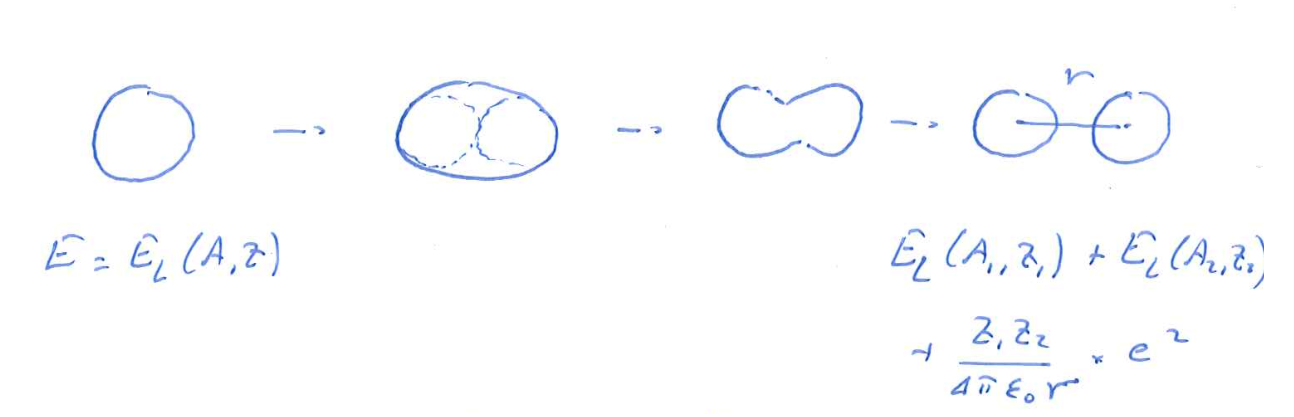
\includegraphics[width=0.8\textwidth]{Figures/nuclear-physics3-fig1}
    \caption{Liquid drop separation as a model of nuclear fission}
    \label{fig:nuclear-physics3-fig1}
\end{figure}

The system can be visualised through a potential, where the nucleus exists if a meta-stable state exists, as represented in Figure \ref{fig:nuclear-physics3-fig2}.
\begin{figure}
    \centering
    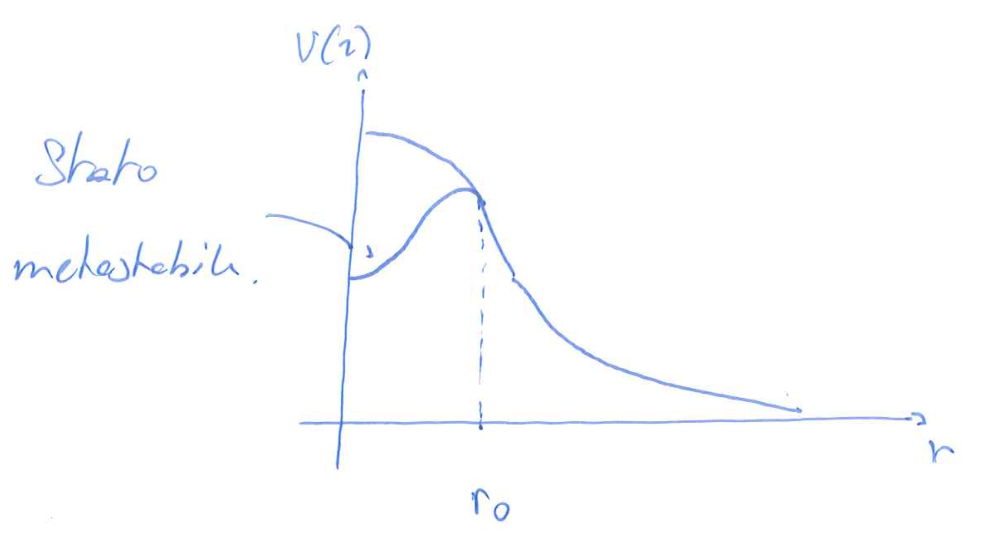
\includegraphics[width=0.8\textwidth]{Figures/nuclear-physics3-fig2}
    \caption{Potential energy as a function of the distance \(r\) from the center of the nucleus.}
    \label{fig:nuclear-physics3-fig2}
\end{figure}
For nuclei with large value of \(A\), the spontaneous fission typically happens promptly, and a meta-stable state does not exist. For some nuclides like $^{238}\mbox{U}$, the spontaneous fission through tunnelling effect can happen, but has an half-life $T_{1/2} \sim 10^{15} \mbox{yr}$.

The spontaneous fission becomes the main process that, probably, forbids the formations of extremely heavy nuclei. 

\subsection{Stability and fission}
Let's represent the deformed nucleus (which is, in the liquid drop model, a sphere) with an ellipsoid of axes \(2a\), \(2b\) and \(2c=2b\), as in Figure \ref{fig:nuclear-physics3-fig3} -- in other words, let the deformation happen along one of the three directions.
\begin{figure}
    \centering
    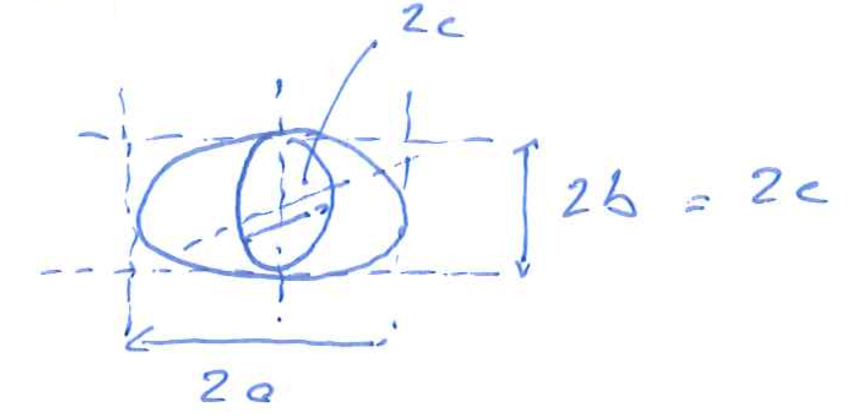
\includegraphics[scale=0.5]{Figures/nuclear-physics3-fig3.pdf}
    \caption{Illustration of the ellipsoid model for Nucleus}
    \label{fig:nuclear-physics3-fig3}
\end{figure}
We assume that the nucleus is incompressible, therefore its volume will remain constant during the deformation:
\begin{equation*}
    V = \frac{4}{3}\pi ab^2 = \frac{4}{3}\pi r^3.
\end{equation*}
The deformations can be parameterized as 
\begin{equation*}
    a = r(1+\epsilon), \;\;\;\;\;\;\;\; b = \frac{r}{\sqrt{1+\epsilon}}.
\end{equation*}
How much would the binding energy change after such deformation?

The volume term in the Bethe Weizs\"acker equation does not change, while the surface term $a_2A^{2/3}$ becomes $a_2A^{2/3}(1+\frac{2}{5}\epsilon^2)$, as the surface of the ellipsoid is given by
\begin{equation*}
    S = 4\pi r^2 \left(1+\frac{2}{5}\epsilon^2\right).
\end{equation*}

The electrostatic energy term is modified in a non-trivial way. One has
\begin{equation*}
    U = \frac{1}{2}\int \int \frac{1}{4\pi\epsilon_0} \frac{\rho(r1)\rho(r2)dr_1dr_2}{r_{12}},
\end{equation*}
an integral which is not trivial, and for the ellipsoid yields
\begin{equation*}
    U = U_{\tiny\mbox{sphere}} \times \left(1-\frac{\epsilon^2}{5}\right),
\end{equation*}
therefore
\begin{equation*}
    a_3 \frac{Z^2}{A^{1/3}} \rightarrow a_3 \frac{Z^2}{A^{1/3}}\left(1-\frac{\epsilon^2}{5}\right),
\end{equation*}
and so
\begin{equation*}
    U = \frac{3}{5}\frac{1}{4\pi\epsilon_0}\frac{Q^2}{R}\left(1-\frac{\epsilon^2}{5}\right).
\end{equation*}

Therefore, after the deformation:
\begin{itemize}
    \item the surface energy term increases;
    \item the electrostatic term decreases.
\end{itemize}
The changes to the Bethe-Weizs\"acker equation are
\begin{equation*}
    a_2A^{2/3}\left(1+\frac{2}{5}\epsilon^2\right)+a_3\frac{Z^2}{A^{1/3}}\left(1-\frac{\epsilon^2}{5}\right) = a_2A^{2/3} + a_3\frac{Z^2}{A^{1/3}} + \left(\frac{2}{5}A^{2/3}a_2 - \frac{a_3}{5}\frac{Z^2}{A^{1/3}}\right) \epsilon^2,
\end{equation*}
and therefore the difference in energy $\Delta E$ between the sphere and the ellipsoid will be
\begin{equation*}
    \Delta E = \frac{2}{5}a_2A^{2/3}\left(1-\frac{a_3}{2a_2}\frac{Z^2}{A}\right) \epsilon^2.
\end{equation*}

The spherical nucleus will be stable if $\Delta E > 0$, and therefore
\begin{equation*}
    \Delta E \sim \frac{2}{5}a_2A^{2/3}\left(1-\frac{1}{50}\frac{Z^2}{A^{1/3}}\right)\epsilon^2.
\end{equation*}
Using the coefficients $a_2$ and $a_3$ discussed before, we find that
\begin{equation*}
    \frac{Z^2}{A} < 50,
\end{equation*}
which holds also for very heavy nuclei. This implies that it is not obvious that nuclei should undergo spontaneous fission.

\subsection{Induced fission}
Through collision with other particles, and in particular with neutrons, the potential barrier of the fission process can be reduced. For the isotope $^{235}\mbox{U}$ the threshold kinematic energy of neutrons to obtain the fission is very low (the same reasoning holds for e.g. plutonium):
\begin{equation*}
    E < 0.1 ~\mbox{eV}.
\end{equation*}
With the capture of a neutron, $^{235}\mbox{U}$ becomes $^{236}\mbox{U}$ which is a even-even nucleus, and therefore has a negative paring term ($a_5$ in the Bethe-Weizs\"acker formula). For  $^{235}\mbox{U}$ this term is null, as \(A\) is odd. The fission threshold for  $^{238}\mbox{U}$ with neutron capture is much  higher, $> 2 ~\mbox{MeV}$.

$^{235}\mbox{U}$ is in the 0.7\% of the natural uranium and undergoes fission with low-energy neutrons, called \emph{thermal}. A neutron is \emph{thermal} when its kinetic energy is comparable to the one of the surrounding atoms (i.e. the neutrons are slowed down to the thermal equilibrium):
\begin{equation*}
    kT = 25 ~\mbox{meV}\,\,\,\,\mbox{at 300 K},
\end{equation*}
where \(k\) is the Boltzmann constant.

$^{235}\mbox{U}$ is the only fissile material with fission induced by thermal neutrons which is significantly abundant in nature. Fissile materials can be produced from fertile materials, as the $^{239}\mbox{Pu}$, $^{233}\mbox{U}$ from the $^{238}\mbox{U}$ and $^{232}\mbox{Th}$. There are auto-fertilizing reactors which burn $^{239}\mbox{Pu}$ and produce $^{239}\mbox{Pu}$ from $^{238}\mbox{U}$.

\begin{figure}[h!]
    \centering
    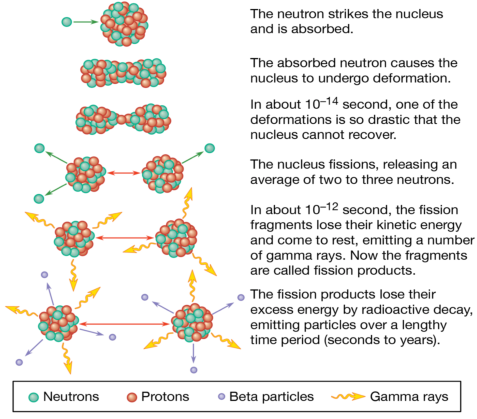
\includegraphics[width=1\textwidth]{Figures/nuclear-physics3-fig4.pdf}
    \caption{Scheme of the induced fission.}
    \label{fig:nuclear-physics3-fig4}
\end{figure}

\begin{figure}
    \centering
    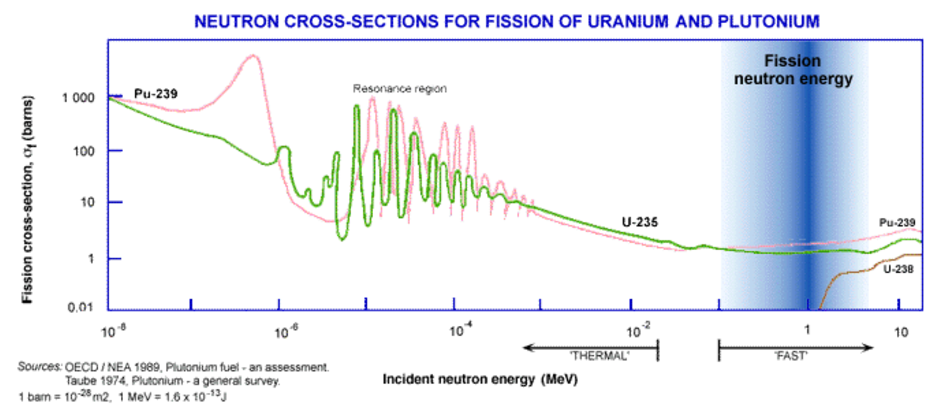
\includegraphics[width=1.\textwidth]{Figures/nuclear-physics3-fig5.pdf}
    \caption{Neutron cross-section for fission of uranium and plutonium}
    \label{fig:nuclear-physics3-fig5}
\end{figure}

\subsection{Chain reactions}
The chain reaction is the base principle of  nuclear reactors:
\begin{equation*}
    \mbox{n} + ^{235}\mbox{U} \rightarrow 
    \mbox{fission products} + 2.5 ~\mbox{neutrons (mean)}
\end{equation*}
For example:
\begin{equation*}
    _{\tiny{0}}^{\tiny{1}}\mbox{n} ~+~ _{\tiny{92}}^{\tiny{235}}\mbox{U}~ \rightarrow~ _{\tiny{92}}^{\tiny{236}}\mbox{U}~ \rightarrow~
    _{\tiny{56}}^{\tiny{141}}\mbox{Ba} ~+~ _{\tiny{36}}^{\tiny{92}}\mbox{Kr} ~+~ 3~_{\tiny{0}}^{\tiny{1}}\mbox{n}.
\end{equation*}
When the nucleus breaks, it generates:
\begin{itemize}
    \item neutrons;
    \item nuclei (and their $\beta$ and $\gamma$ decays) with kinetic energy which generates heat in the material; 
    \item additional neutrons emitted by the produced nuclei, called \emph{delayed neutrons}.
\end{itemize}
Produced neutrons can also be captured by other nuclei and produce a chain reaction, as represented in Figure \ref{fig:nuclear-physics3-fig6}.

\begin{figure}
    \centering
    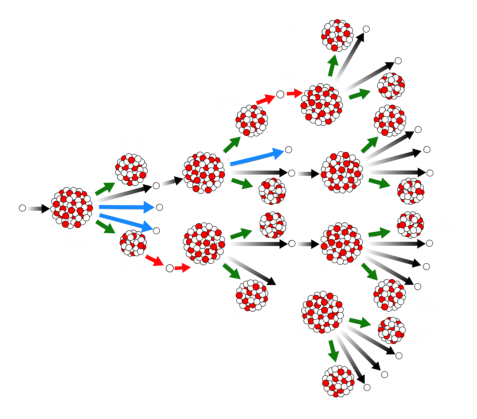
\includegraphics[scale=1.2]{Figures/nuclear-physics3-fig6.pdf}
    \caption{Chain reaction. The blue arrows indicate the late emission of neutrons. The red arrows indicate the capture of neutrons by other nuclei.}
    \label{fig:nuclear-physics3-fig6}
\end{figure}

A fundamental aspect of the chain reaction is its control:
\begin{itemize}
    \item an insufficient production of neutrons stops the chain;
    \item an over-production of neutrons leads to an exponential process which lead to the \emph{explosion} of the system.
\end{itemize}

The reaction chain can be modelled in terma of a few parameters:
\begin{itemize}
    \item \(N(t)\): number of neutrons at time \(t\);
    \item $\tau$: mean time for a neutron to produce a primary fission;
    \item $\nu$: mean number of neutrons produced in a fission process;
    \item \(q\): probability for a neutron to produce a fission (taking into account the absorbed neutrons which do not produce any fissions).
\end{itemize}

For each passage from the \(i\)-th step of the chain reaction, called \emph{generation}, to the \(i+1\)-th, we have a variation \(dN\) in the number of neutrons, which can be written as
\begin{equation}
    \frac{\mbox{dN}}{\mbox{N}} = \lambda (-1 + \nu q)~dt
    \label{eq:nuclear-physics3-eq1}
\end{equation}
where the \(-1\) is due to the primary fission while the term $\nu q$ accounts for the effective number of neutrons which contribute to the chain. If we integrate and use $\lambda=\frac{1}{\tau}$ we obtain
\begin{equation*}
    \mbox{N}(t) = \mbox{N}(0)~ e^{(\nu q -1)\frac{t}{\tau}},
\end{equation*}
where:
\begin{itemize}
    \item for $\nu q < 1$ the regime is called \emph{sub-critical}, and the chain reaction does not develop: the number of neutrons decreases with time;
    \item for $\nu q = 1$ the regime is called \emph{critical}, and the number of neutrons (and secondary fission processes) is stable;
    \item for $\nu q > 1$ the regime is called \emph{super-critical}, and the number of reactions increases exponentially.
\end{itemize}

\subsection{Cross section and critical mass}
The neutrons generated in the fission process can undergo several processes:
\begin{itemize}
    \item they can be captured by other nuclei, emitting $\gamma$ radiation (without producing fission) -- a process with a cross-section $\sigma_{n,\gamma}$;
    \item they can undergo elastic scattering or lose energy through inelastic scattering processes;
    \item they can produce a new fission -- a process with a cross-section $\sigma_{\tiny\mbox{fission}}$.
\end{itemize}

Typically neutrons lose energy through collisions. The factor $q$ in Equation \ref{eq:nuclear-physics3-eq1} can be written as 
\begin{equation}
    q = \frac{\bar{\sigma}_{\tiny\mbox{fission}}}{\bar{\sigma}_{\tiny\mbox{fission}} + \bar{\sigma}_{n,\gamma}}.
\end{equation}

For $^{238}\mbox{U}$ and $T_{\tiny\mbox{neutron}} = 2~\mbox{MeV}$:
\begin{itemize}
    \item $\sigma_{\tiny{\mbox{tot}}} = 7.3~\mbox{b}$;
    \item $\sigma_{\tiny{\mbox{fission}}} = 0.53~\mbox{b}$;
    \item $\sigma_{n,\gamma} = 0.048~\mbox{b}$.
\end{itemize}
Therefore, most of the collisions are scatterings with loss of energy in which the neutron is not absorbed.

For  $^{235}\mbox{U}$, again with $T_{n} = 2~\mbox{MeV}$, the picture is similar:
\begin{itemize}
    \item $\sigma_{\tiny{\mbox{tot}}} = 7.15~\mbox{b}$;
    \item $\sigma_{\tiny{\mbox{fission}}} = 1.89~\mbox{b}$;
    \item $\sigma_{n,\gamma} = 0.059~\mbox{b}$.
\end{itemize}
\begin{figure}
    \centering
    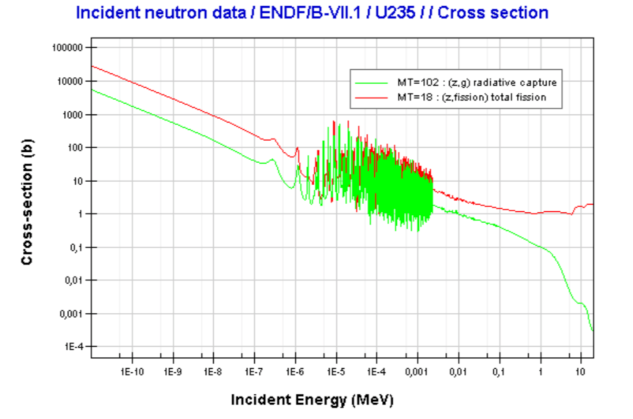
\includegraphics{Figures/nuclear-physics3-fig7.pdf}
    \caption{Cross section as a function of incident energy for $^{235}\mbox{U}$.}
    \label{fig:nuclear-physics-fig7}
\end{figure}

The situation totally changes for thermal neutrons with a kinematic energy of \SI{25}{meV}. 
\begin{table}[]
    \centering
    \begin{tabular}{|c|c|c|c|}
         \hline
         & $\sigma_{\tiny{\mbox{tot}}}$ & $\sigma_{\tiny{\mbox{fission}}}$ & $\sigma_{n,\gamma}$ \\
         \hline
        $^{235}\mbox{U}$ & 703 b & 589 b & 95 b \\
        \hline
        $^{238}\mbox{U}$ & 12 b & $2\cdot10^{-5}$ b & 2.7 b \\
        \hline
    \end{tabular}
    \caption{Summary table of cross sections for two isotopes of uranium (for neutrons of \SI{25}{meV})}
    \label{tab:nuclear-physics3-tab1}
\end{table}
For neutrons of \SI{2}{MeV}, the cross section is low for both $^{235}\mbox{U}$ and $^{238}\mbox{U}$. However, for $^{235}\mbox{U}$ and $T_{n} = 25~\mbox{meV}$ the cross section is two orders of magnitude higher.
For energies lower than \SI{2}{MeV} (fission threshold of  $^{238}\mbox{U}$) the condition $q\ll 1$ is easily verified, since the neutrons are mainly subject to scattering without any absorption process, and therefore they lose energy.

$T_{n} = 2~\mbox{MeV}$ is exactly the mean kinetic energy of the neutrons emitted through the fission process. 
\begin{figure}
    \centering
    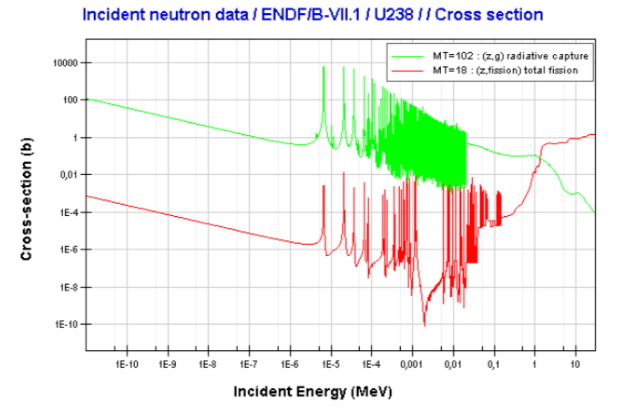
\includegraphics{Figures/nuclear-physics3-fig8.pdf}
    \caption{Cross section as a function of incident energy for $^{238}\mbox{U}$.}
    \label{fig:nuclear-physics-fig8}
\end{figure}

\subsection{How nuclear reactors work}
A nuclear reactor is typically composed by the following elements:
\begin{itemize}
    \item \emph{combustible}: contains $^{235}\mbox{U}$ and $^{238}\mbox{U}$;
    \item \emph{absorber}: material to absorb neutrons (boron, argon, cadmium);
    \item \emph{moderator}: material to thermalise neutrons (H$_2$O, graphite, beryllium);
    \item \emph{heat exchanger}: a means to exchange heat and transfer it, in order to generate electric current.
\end{itemize}

Through several reactions and absorptions it is possible to maintain the reactor in the \emph{critical} state, meaning that the reaction is controlled and the system in stable. The critical regime is the normal functioning state of a reactor. 

The critical regime is also related to the mean path of the neutrons before they are captured or initiate another fission process. Therefore, there is a minimum distance needed for the reaction to self-sustain, and therefore there a critical volume, or  \emph{critical mass}, which can be evaluated. This critical mass is controlled through the use of the absorbers, which are used to control the chain reaction.

\begin{figure}
    \centering
    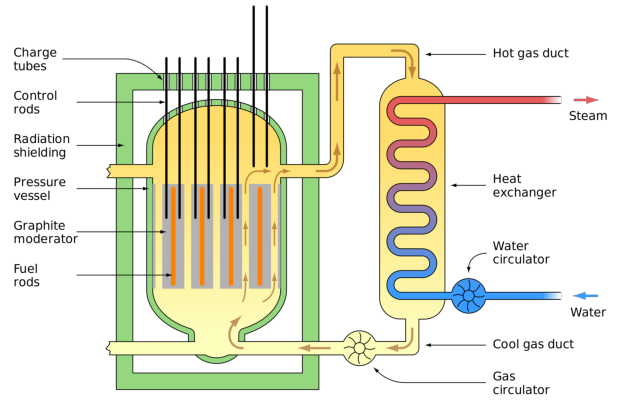
\includegraphics{Figures/nuclear-physics3-fig9.pdf}
    \caption{Scheme of a nuclear reactor with: gas (CO$_2$) heat exchanger, natural uranium as combustible, boron as absorber, graphite as moderator element.}
    \label{fig:my_label}
\end{figure}

\section{Nuclear fusion}
The behaviour of the binding energy per nucleon for \(A<60\) suggests that another process may be favoured to bring two light nuclei into a more stable final state, \emph{fusion}, which can be written in general as
\[
_z^aX + _{Z-z}^{A-a} \to _{Z}^AN + Q,
\]
where \(Q\) represents the corresponding release of energy.

As \(^2H\) is the only stable bound state formed by two nucleons, the simplest fusion process is
\begin{equation*}
    p~+~p \rightarrow ^{2}\mbox{H}~+~e^{+} + \nu_e.
\end{equation*}
Fusion happens in general when \(A<60\), as the fusion product must be stable.
Figure \ref{fig:nuclear-physics3-fig10} shows two examples of basic fusion processes, the deuterium-deuterium reactions (\emph{D-D reactions}). Their final states include a neutron or a proton that take about \(75\%\) of the total available kinetic energy in the reaction, which is of the order of \SI{4}{MeV}. The more stable the nucleus produced in the fusion process, the higher the \(Q\)-value of the reaction: the process
\[
^2H+^3H\to _2^4He+n,
\]
where an \(\alpha\) particle is produced, has a \(Q\)-value of about \SI{17.6}{MeV}, and can be regarded as a source of fast neutrons.

In general, a fusion process can happen only if the two initial state nuclei can overcome the Coulombian potential barrier (i.e. the repulsion between their protons) and form a bound state. If we consider nuclei as spheres, the distance between the nuclei when they are in contact (and fusion occurs) can be approximated as $2\times R=2R_0\times A^{1/3}$, so to have the fusion process \(X+Y\to N\)% (keep in mind that the weak nuclear force acts on distances of the order $~10^{-18}~\mbox{m}$).
one needs enough energy to win the electromagnetic repulsion, i.e.
\begin{equation*}
    V_{XY} = \alpha\frac{\hslash c}{2R}Z_{x}Z_{y},
\end{equation*}
which in the case of \(X=Y=p\) is \(V_{pp}\sim 0.7 ~\mbox{MeV}\).

The nuclear fusion is the process active in our Sun -- a star mostly composed by hydrogen (a source of ``proton fuel''!) -- which produces energy. Since the temperature at the center of the Sun is $T \sim 15 \times 10^6~\mbox{K}$, the mean energy of the protons will be 
\begin{equation*}
    kT \sim \SI{1.3}{keV},
\end{equation*}
which is about \(600\) times less than the energy needed to overtake the \(pp\) potential barrier. The \(pp\) fusion process must therefore happen through quantum tunneling: if we consider the protons inside the Sun as a gas of protons, their velocity distribution will follow a Maxwellian distribution,
\[
\frac{dN}{dv} = \frac{v^2}{\left(2kT/m_p\right)^{3/2}}e^{-\frac{m_pv^2}{2kT}},
\]
where \(k\) is the Boltzmann constant\footnote{In natural units one has \(kT=\SI{25}{meV}\) for room temperature.}, \(T\) the temperature of the proton gas and \(m_p\) is the proton mass.
It will be the protons in the tails of this distribution which will have a chance to undergo tunneling, overcome the Coulomb barrier and undergo fusion. The treatment of this process is similar to the Gamow theory of $\alpha$ decays, i.e. the tunneling probability will be \(\propto\exp(-2G)\), where \(G\) is the Gamow factor for fusion.

\subsection{Fusion processes in the Sun}
The fusion processes in the Sun are induced by two main \emph{cycles}, i.e. cyclic processes where hydrogen contained in the Sun acts as a fuel, with the emission of energy:
\begin{itemize}
    \item the \(pp\) cycle (proton-proton chain) transforms protons into helium: this cycle, which starts with the process \(p+p\to^2H+e^++\nu_e\) (which is the bottleneck of the cycle, as it happens about \(10^{-18}\) times per second per proton\footnote{This is a weak-interaction process!}), is made by several branches which go through heavier elements like beryllium or boron, but end in helium (see Fig. \ref{fig:nuclear-physics3-fig11});
    \item the CNO cycle, which uses carbon contained in the Sun as a catalyst\footnote{This means that the net amount of carbon after one cycle is the same: its presence is only needed for the cycle to happen.} to produce \(^{4}He\) with the provision of a total of \(4\) protons, through the following reactions (see Fig. \ref{fig:nuclear-physics3-fig12}):
    \begin{equation*}
    \begin{split}
        &^{12}C~+~p ~ \rightarrow ~ ^{13}\mbox{N}~+~\gamma + 1.95~\mbox{MeV}\\
        &^{13}N ~ \rightarrow ~ ^{13}\mbox{C}~+~ e^+ ~+~ \nu_e ~+~ 1.37~\mbox{MeV}\\
        &^{13}C ~+~p \rightarrow ~ ^{14}\mbox{N}~+~\gamma + 7.94~\mbox{MeV}\\
        &^{14}N ~+~p \rightarrow ~ ^{15}\mbox{O}~+~\gamma + 7.39~\mbox{MeV}\\
        &^{15}O ~\rightarrow ~ ^{15}\mbox{N}~+~ e^+ + \nu_e + 1.86~\mbox{MeV}\\
        &^{15}N ~+~ p ~\rightarrow ~ ^{12}\mbox{C}~+~ ^{4}\mbox{He} + 4.96~\mbox{MeV}\\
    \end{split}
    \end{equation*}
\end{itemize}
These reactions all produce energy and neutrinos, as they can be summarised as
\begin{itemize}
    \item \(pp\) cycle: \(4p\to ^2He+2p\);
    \item \(CNO\) cycle: \(4p\to ^4He+2e^++2\nu_e\) 
\end{itemize}
with a release of energy \(Q\sim\SI{25}{MeV}\). 

\begin{figure}
    \centering
    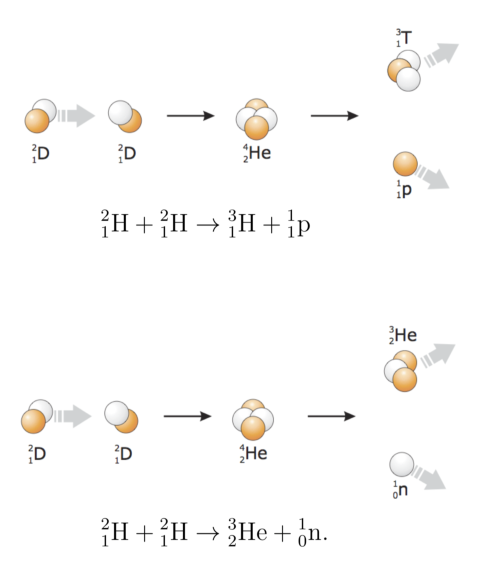
\includegraphics[width=0.8\textwidth]{Figures/nuclear-physics3-fig10.pdf}
    \caption{}
    \label{fig:nuclear-physics3-fig10}
\end{figure}

\begin{figure}
    \centering
    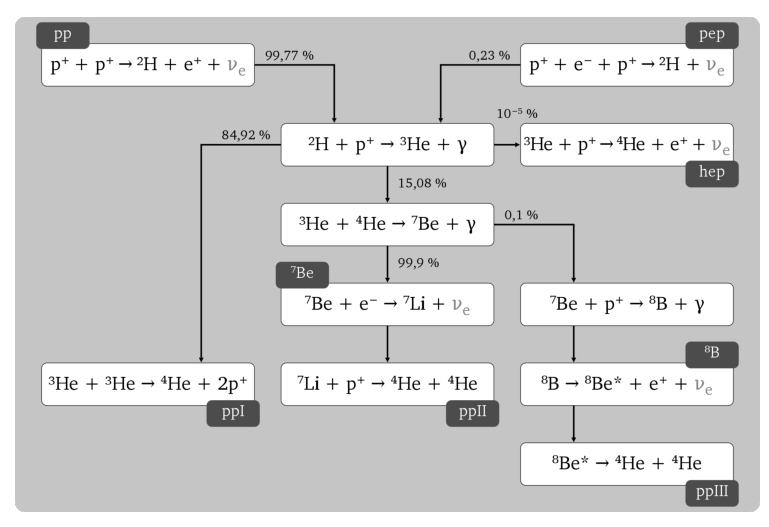
\includegraphics[width=0.8\textwidth]{Figures/nuclear-physics3-fig11.pdf}
    \caption{}
    \label{fig:nuclear-physics3-fig11}
\end{figure}

\begin{figure}
    \centering
    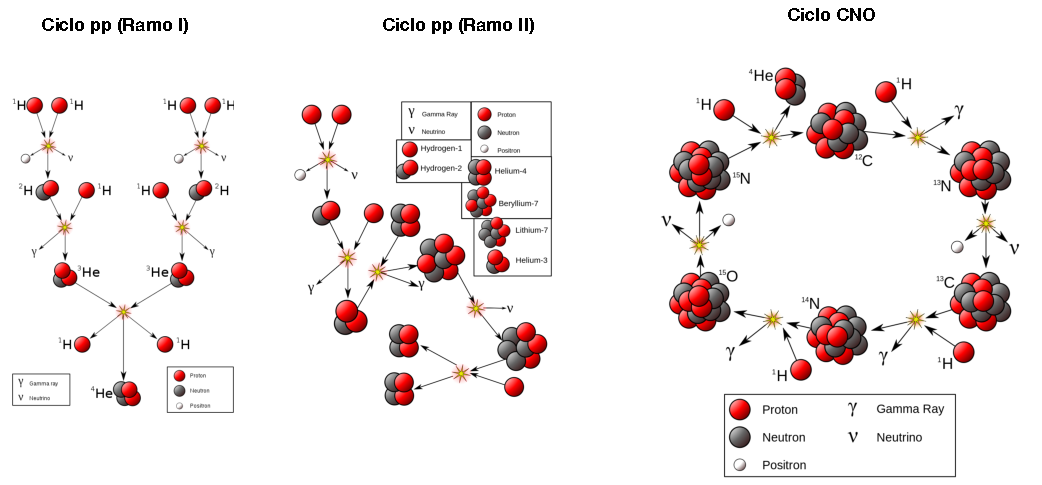
\includegraphics[width=0.8\textwidth]{Figures/nuclear-physics3-fig12.pdf}
    \caption{}
    \label{fig:nuclear-physics3-fig12}
\end{figure}


\section*{Take-home lessons}
\begin{itemize}
    \item An estimation of the size of atomic nuclei can be obtained from the typical kinetic energy of $\alpha$ particles, from which one can derive their momentum and -- through Heisenberg's indetermination principle -- the size of the nucleus.
    \item There are in general different possible ways to measure the radius of nuclei. For example, by measuring the differential scattering cross section with electrons as a function of the transferred momentum, one can extract the spatial distribution of the charges in the nucleus. Or, one can measure the emission spectrum of $X$ rays by atomic electrons, and use the fact that the internal orbitals are influenced by the finite dimension of nuclei. Similar results are obtained, which indicate that the nucleus can be approximated with a sphere with a volume proportional to the atomic mass number $A$: the radius of the nucleus is therefore $R=R_0 A^{1/3}$, with $R_0\approx \SI{1.2}{fm}$.
    \item The \emph{binding energy} $E_L$ of a nucleus is given by the difference between its mass $M(A,Z)$ and the sum of masses of its constituents ($Z$ protons and $A-Z$ neutrons). For $A>12$, the ratio $E_L/A$ is almost constant (\SI{8}{MeV} per nucleon).
    \item The atomic mass $m(A,Z)$ includes the mass of the electrons and their binding energy, $m(A,Z)=M(A,Z)+Zm_e-B_e(Z)/c^2$. The mass excess is defined as the difference between $m(A,Z)$ and $A \si{u}$, where $\SI{1}{u}=m(^{12}C)/12$.
    \item Nuclear interactions are short-ranged. Nucleons interact mostly with their first neighbours; adding another nucleon does not cost more than the previous ones, in the sense that the total energy (the binding energy) is proportional to the number of particles, $E_L\propto A$. This is different from long-range interactions like the Coulomb interaction, where a particle interacts with all particles and $E_{n+1}\propto E_n$, and the binding energy is $E_L\propto A(A-1)$.
    \item A first model of atomic nucleus is the \emph{liquid drop} model, which -- similarly to water drops which are held together by inter-molecular forces -- assumes that the nucleus is an incompressible sphere with radius $R\propto A^{1/3}$ and that the interaction is short-ranged. The binding energy is parameterised by the Bethe-Weizsaecker formula, $E_L(A,Z) = -a_1 A + a_2 A^{2/3} + a_3 Z^2/A^{1/3} + a_4 (A-2Z)^2/A \pm a_5 A^{-3/4}$. The term multiplied by $a_1$ accounts for the fact that the interaction is short-ranged, so that nucleons inside the sphere have bindings in all directions with their first neighbours. The term multiplied by $a_2$ is a surface term, which takes into account the fact that external nucleons have only bindings with the internal part. The term multiplied by $a_3$ accounts for the Coulomb electrostatic repulsion between protons. The term multiplied by $a_4$ takes into account the quantization of the energy levels and the Pauli exclusion principle. The term multiplied by $a_5$, or \emph{pairing term}, is related to the magnetic interaction between nucleons. By minimizing the Bethe-Weizsaecker formula, one can find the relation between $Z$ and $A$ which defines the \emph{stability valley}, which for small $A$ includes elements for which $Z\approx A/2$, and for high $A$ those which have $Z\approx 2a_4/a_3 A^{1/3}$.
    \item The Fermi gas model, instead, assumes that protons and neutrons are confined in a pothole with spherical symmetry with the size of the nuclear radius $R=R_0 A^{1/3}$. The pothole is a box for neutrons, while in the case of protons the potential outside it follows the Coulomb dependence on radial distance from the nucleus center. From the corresponding density of states, one can compute the momentum and energy (\emph{Fermi energy}) of nucleons, which for elements with $Z\approx A/2$ are of about \SI{250}{MeV/c} and \SI{33}{MeV}, respectively.
    \item The shell model is based on the Bohr-Sommerfeld atomic model, which uses a Coulomb potential with spherical symmetry, centered around the nucleus, and includes the quantization of angular momentum and respects the Pauli exclusion principle. Energy levels are defined by three quantum numbers ($n, l, m$). In analogy to the atomic model (and with differences related to the difficulty of defining an analogous of electron orbitals), one can develop a shell model of the \emph{nucleus}, where protons and neutrons are treated as two different isospin eigenstates of the same particle, the nucleon.
    \item Experiments show that there are a few particularly stable elements, i.e. with a large binding energy, that have a specific number of neutrons. These numbers of neutrons form the so-called \emph{nuclear magic numbers}, which are observed to be $2, 8, 20, 28, 50, 82, 126$: the better a model of the nucleus, the more magic numbers are "explained" by its predictions.
    \item The complex theoretical task is that of finding a nuclear potential which is able to explain as many magic numbers as possible. An harmonic potential is able to explain only a few of them; the Woods-Saxon potential, which depicts the nucleus as a "smooth" 3D box, isn't fully accurate as well. Meyer and Jensen found that, in order to find predicted magic numbers which match the observed magic numbers, one needs to include a term analogous to the spin--orbit interaction in atomic physics, which isn't however of electromagnetic nature. This induces a splitting of energetic levels, which reproduces the observed magic numbers.
    \item The term proportional to $a_4$ in the Bethe-Weizsaecker formula takes into account the symmetry between protons and neutrons, for which the most stable configuration is the one in which the number of protons and neutrons in a nucleus are identical.
    The term proportional to $a_5$, instead, takes into account the fact that two neighbouring nucleons have spin-spin interactions, which leads to the so-called pairing energy, favouring the case of unaligned spins. Nuclei with $Z$ and $N=A-Z$ which are bot even, have a fundamental state with spin zero.
    \item Nuclear fission is a spontaneous process in which a nucleus transforms in different fragments. An example are $\alpha$ decays, which happens due to the tunneling through the short-range potential barrier of the nuclear interaction. Fission happens when the atomic number of an element is large, so that the electrostatic repulsion between nucleons becomes strong. Fission can be visualized as the splitting process of a liquid drop. It can be modelled by considering the nucleus as described by a potential, which determines whether a given state of a nucleus exists (as a meta-stable state) or not: the higher the tunneling probability, the lower the lifetime of the nucleus. In order to determine the stability conditions of a nucleus, one can represent it as an incompressible ellipsoid and compute the difference in binding energy with respect to an undeformed sphere. One finds that the stability condition is $Z^2/A<50$, which is verified for most nuclei.
    \item If one scatters other particles (e.g. neutrons) with nuclei, the potential barrier of fission reduces and fission may be induced. Depending on the nucleus, the threshold kinetic energy may be as low as \SI{0.1}{eV} ($^{235}U$), which requires \emph{thermal neutrons}, i.e. neutrons whose kinetic energy is comparable to the one of the surrounding atoms ($kT\approx\SI{25}{meV}$ at \SI{300}{K}). One can also induce chain reactions, as fissions usually produce neutrons and other nuclei: while these nuclei may decay to a ground state with the emission of photons, or undergo radioactive decays, the additional neutrons could induce other fissions, or be captured by nuclei which then produce $\gamma$ radiation, or undergo elastic or inelastic scattering. Chain reactions can be described with a simple mathematical model, which identifies a sub-critical, a critical and a super-critical regime, which correspond to decreasing, stable and increasing number of neutrons as a function of time, depending on the mean number of neutrons produced in a fission process and on the probability of those neutrons to produce a fission. Nuclear reactors exploit the critical regime, using $^{238}U$ or $^{235}U$ as fuel, a neutron absorber, a moderator to thermalise neutrons and a heat exchanger to transfer the heat released in the chain reaction processes into electric current. As the critical regime depends on the free mean path of neutrons before being captured or undergoing fission, there is a minimal distance which is necessary to allow the self-sustain of the chain reaction, which corresponds to a critical volume (or \emph{critical mass}), which is controlled with neutron absorbers.
    \item Fusion processes, like $p+p\to ^{2}H + e^+ + \nu_e$, happen naturally in stars. In order for the two protons to fuse together in a bound state, one needs them to overcome a Coulombian potential barrier with a size of $\approx \SI{1}{fm}$ (higher than the range of the weak interaction which allows charge exchange, \SI{1e-18}{m}), corresponding to about \SI{0.7}{MeV}. Since the temperature at the center of the Sun is about \SI{15e6}{K}, the average energy of protons is $kT\approx\SI{1.3}{keV}$ i.e. much lower than the potential barrier: also the fusion process therefore happens thanks to the tunneling effect.
    \item Fusion processes in the Sun happen mostly due to two main cycles, the \emph{$pp$ cycle} which transforms protons in helium after passing through more complex nuclei, and the \emph{CNO} cycle which starts from carbon and allows to produce $^4He$ by providing a total of $4$ protons. All of these reactions imply the release of energy, and the production of neutrinos.
\end{itemize}
\section*{Questions}
\begin{itemize}
    \item 
\end{itemize}